\documentclass[14pt]{beamer} %Makes presentation

\setbeamersize{text margin left=1em,text margin right=1.75em}
\setbeamertemplate{frametitle}[default][center]
\setbeamerfont{frametitle}{size=\large}
\setcounter{tocdepth}{1}

% packages
\usepackage{bbding,multirow,times,ccaption,tabularx,graphicx,verbatim,booktabs} %graphics,
\usepackage{color}
\usepackage{colortbl}%Table overlays
\usepackage[english]{babel}

%% white on black
%\setbeamercolor{normal text}{fg=white,bg=blue!20!black}
%\setbeamercolor{structure}{fg=white, bg=blue!20!black}
%\setbeamercolor{alerted text}{fg=yellow!70!orange}
%%\setbeamercolor{item projected}{use=item,fg=black,bg=item.fg!35}
%\setbeamercolor*{palette primary}{use=structure,fg=structure.fg}
%\setbeamercolor*{palette secondary}{use=structure,fg=structure.fg!95!black}
%\setbeamercolor*{palette tertiary}{use=structure,fg=structure.fg!90!black}
%\setbeamercolor*{palette quaternary}{use=structure,fg=structure.fg!95!black,bg=black!80}
%\setbeamercolor*{framesubtitle}{fg=white}
%\setbeamercolor*{block title}{use=structure, bg=blue!20!black}
%\setbeamercolor*{block body}{use=structure}

% black on white
\usetheme{Singapore} %Gray with fade at top
\usecolortheme{seagull} %Color theme
\usecolortheme{rose} %Inner color theme
\setbeamercolor{item}{fg=black!65}
\setbeamercolor{enumerate item}{fg=black!55}

% LSE branded background
\setbeamertemplate{background}
{
\includegraphics[height=\paperheight,keepaspectratio]{images/lse2.png}}

%\useoutertheme[subsection=false]{miniframes} %Supppress subsection in header
\useinnertheme{rectangles} %Itemize/Enumerate boxes
\setbeamertemplate{navigation symbols}{}
%\setbeamertemplate{mini frames}[default]
%\setbeamercovered{dynamics}
\setbeamerfont*{title}{size=\Large,series=\bfseries}
%\setbeamertemplate{headline}{}

\usepackage{tikz}
\usetikzlibrary{shapes,arrows}

\usepackage{multicol}

\newcommand{\heading}[1]{\noindent \textbf{#1}\\ \vspace{1em}}

\newcommand{\hltfootnote}{
\vspace{1em}
\footnotesize{Source: Hobolt, Leeper, and Tilley (YouGov)}
}

% font
\usepackage{tgadventor}
\renewcommand*\familydefault{\sfdefault} %% Only if the base font of the document is to be sans serif
\usepackage[T1]{fontenc}

\title[]{{\large Brexit: What happened? What now?}}

\author{
Dr Thomas J. Leeper
}

\date[]{{\footnotesize 13 March 2018\\Research funded by ESRC \textit{UK in a Changing Europe} Initiative}}

\begin{document}

\bgroup
\setbeamercolor{background canvas}{bg=white}
\begin{frame}[plain]
\begin{center}

\includegraphics[height=.9\textheight]{images/lse-beaver}
\end{center}
\end{frame}
\egroup

\frame{}

\frame{\titlepage}

\frame{
\frametitle{About Me}

\begin{itemize}\itemsep1em
\item Associate Professor at LSE (since 2015)
\item Postdoc at Aarhus University (2012--2015)
\item PhD from Northwestern University (2012)
\end{itemize}
}



\frame{}

\frame{\tableofcontents}


\section{Background and Campaign}
\frame{\tableofcontents[currentsection]}

\frame{

``If there was a referendum on your country's membership of the EU, how would you vote?''

\begin{center}
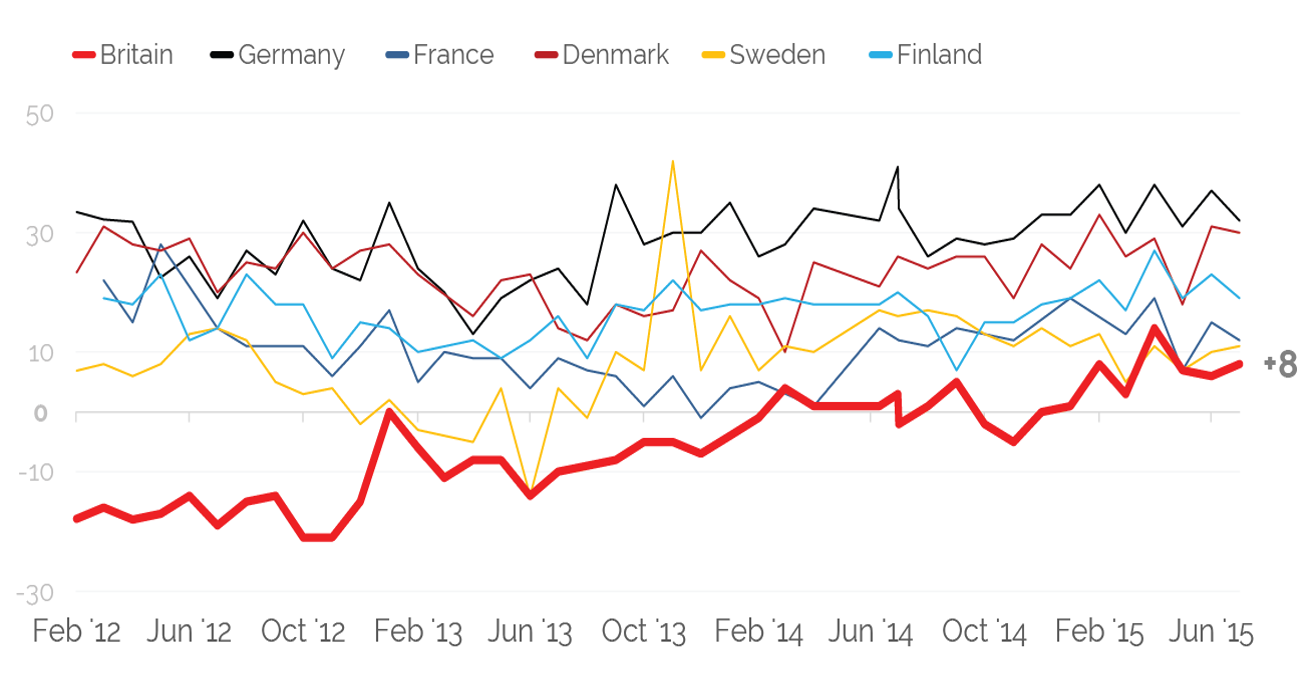
\includegraphics[width=\textwidth]{images/yougov-referendum-by-country.png}

\end{center}

\vspace{1em}

{\footnotesize Source:  YouGov, July 2015}

}


\frame{
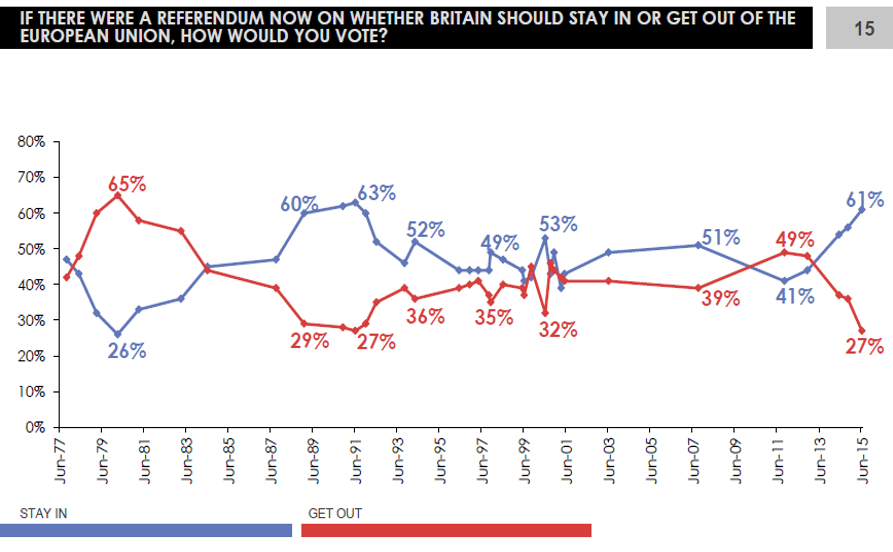
\includegraphics[width=\textwidth]{images/ipsos-mori-trend.png}
\vspace{1em}
\footnotesize{Source: Ipsos MORI}
}

\frame{
\begin{center}
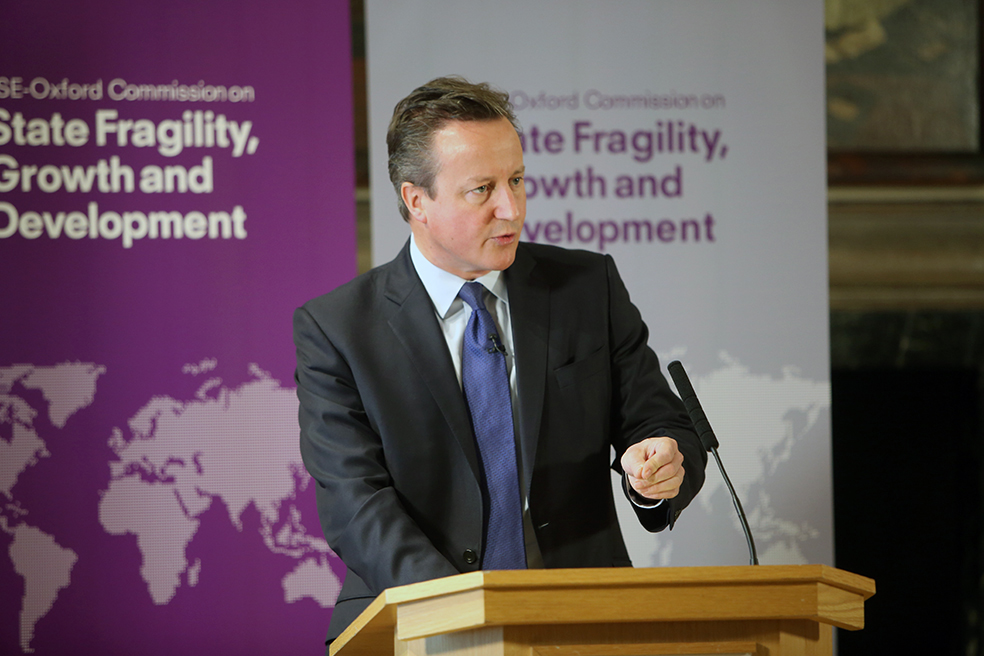
\includegraphics[width=\textwidth]{images/david-cameron.png}
\end{center}
}


\frame{
\begin{center}
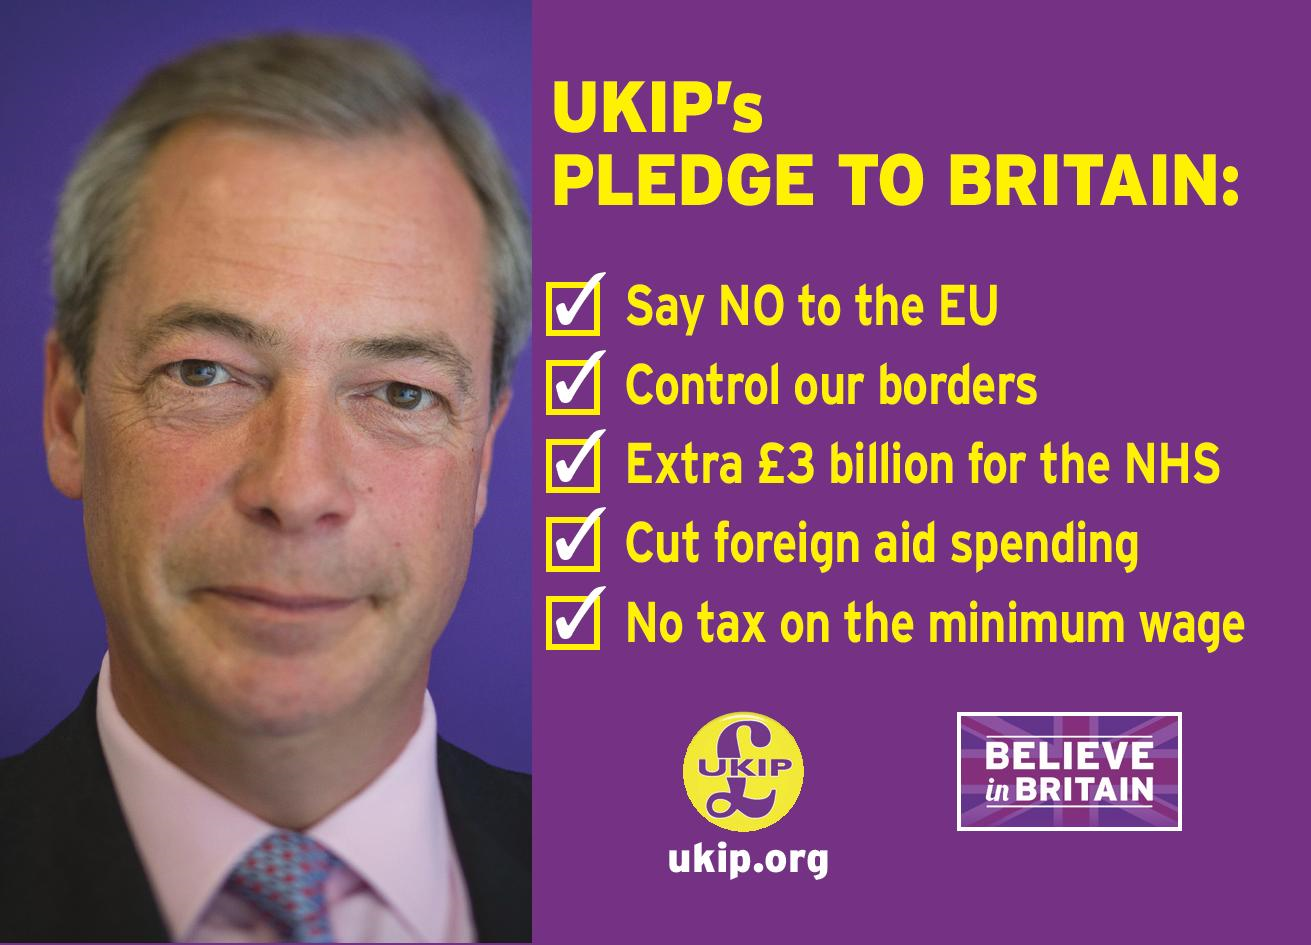
\includegraphics[height=.8\textheight]{images/ukip-pledge.png}
\end{center}
}

\frame{
\begin{center}
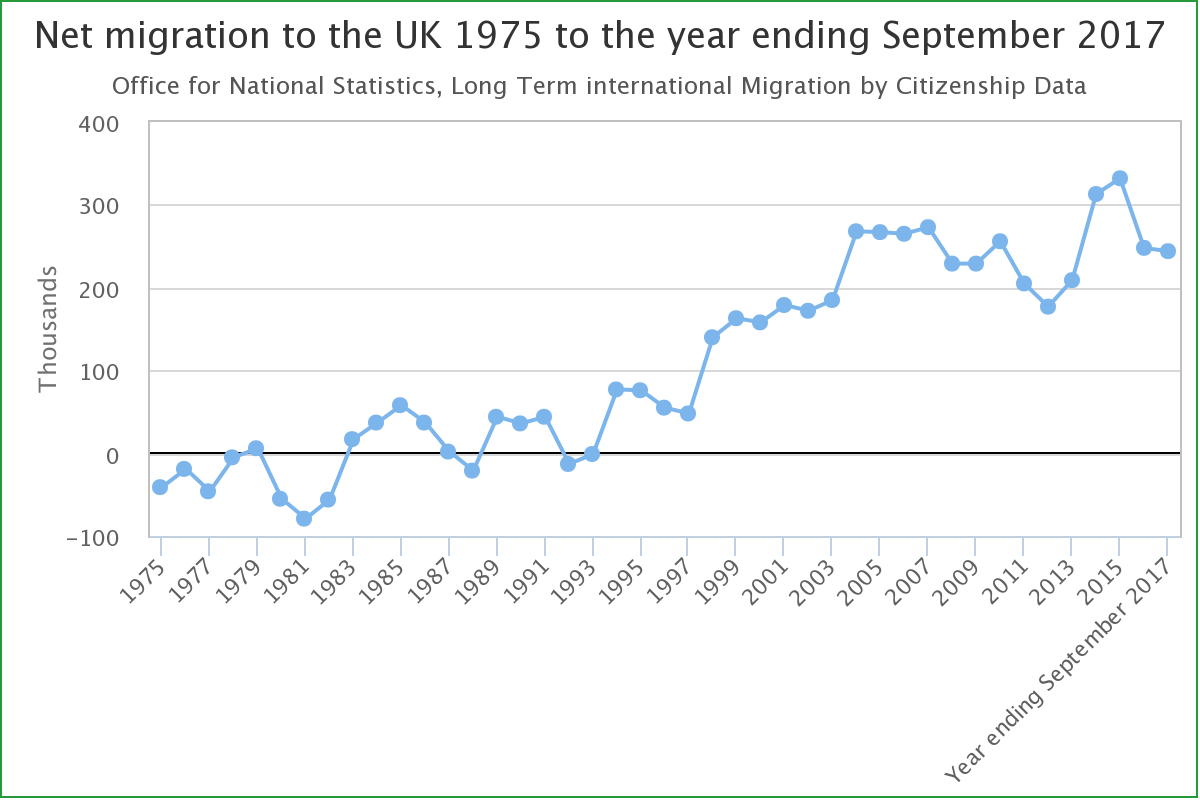
\includegraphics[width=.9\textwidth]{images/net-migration-trend.png}
\end{center}
}


\frame{
\begin{center}
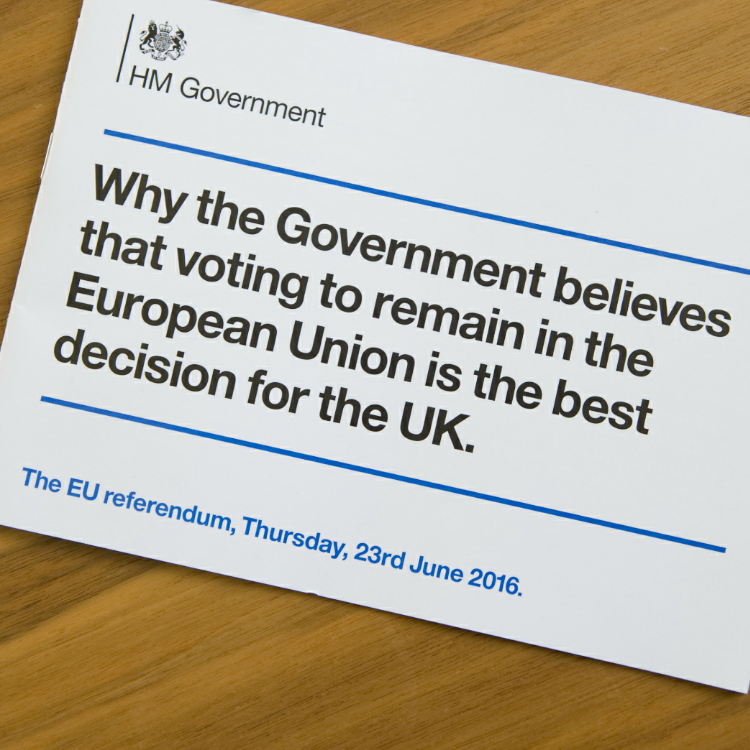
\includegraphics[height=\textheight]{images/government-leaflet.png}
\end{center}
}

\frame{
\begin{center}
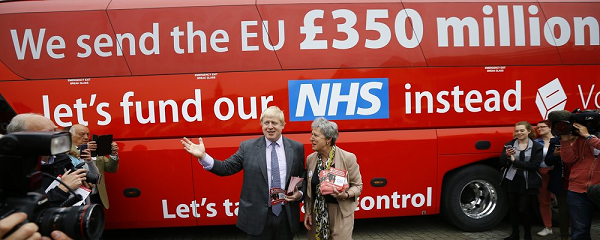
\includegraphics[width=\textwidth]{images/brexit-bus.png}
\end{center}
}


\frame{
\begin{center}
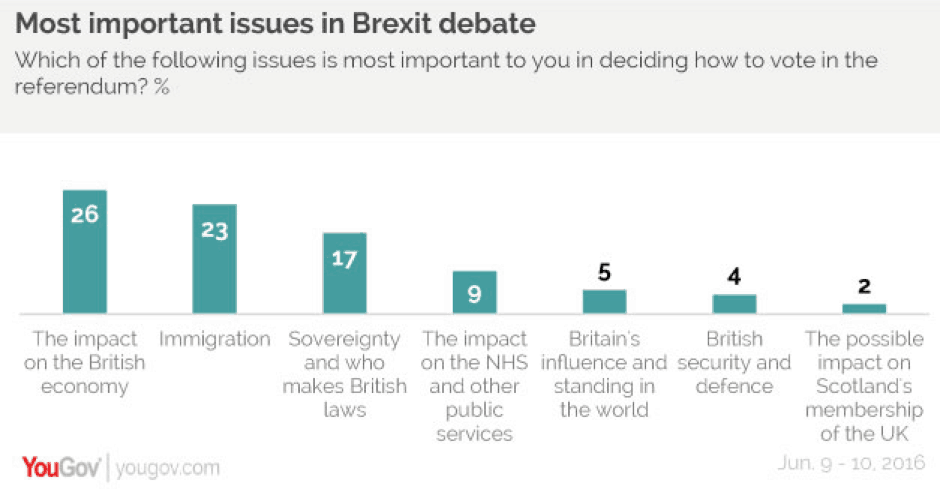
\includegraphics[width=\textwidth]{images/brexit-issue-priorities.png}
\end{center}
}



\frame{
\begin{center}
\colorbox{white}{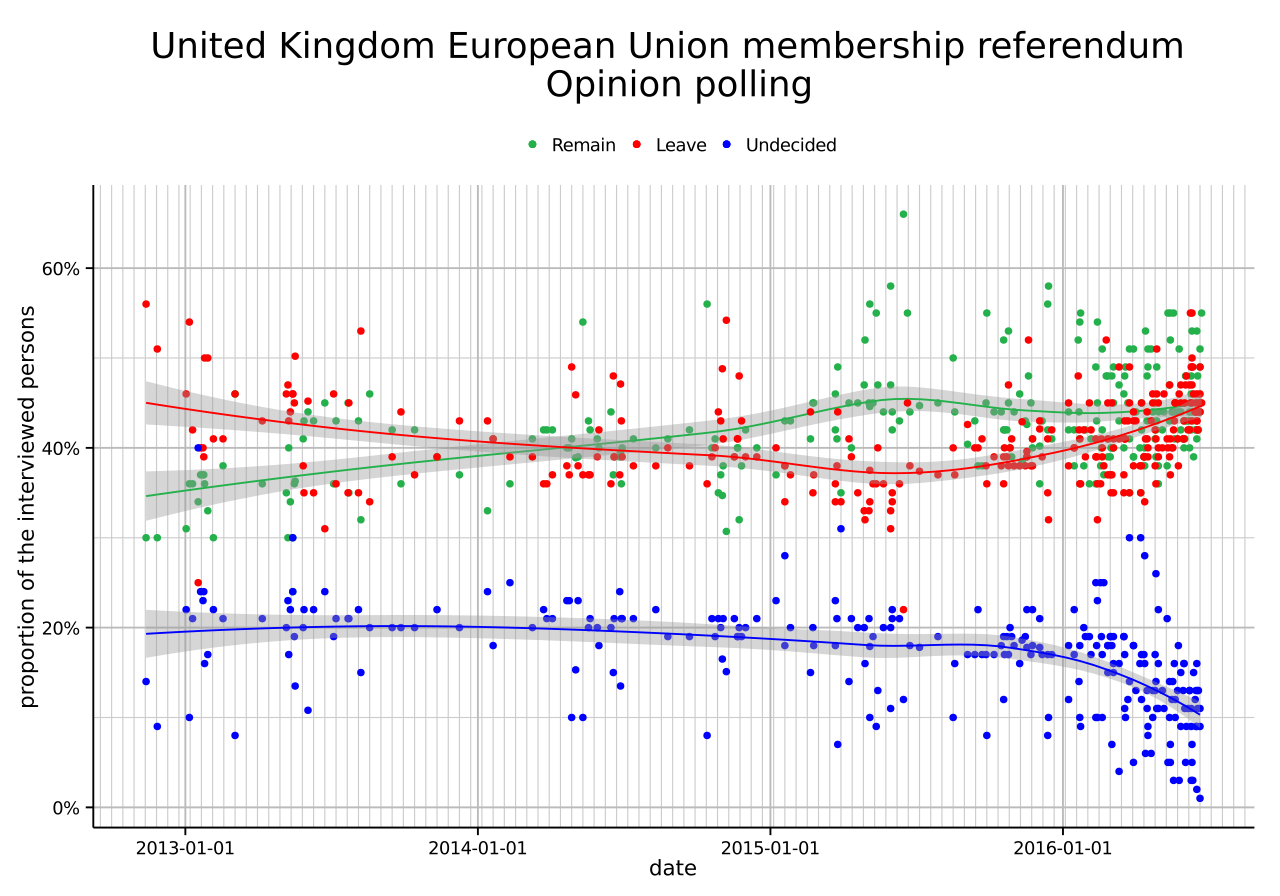
\includegraphics[width=\textwidth]{images/referendum-polling.png}}
\end{center}
}


\section{The Result}
\frame{\tableofcontents[currentsection]}

\frame{
\begin{center}
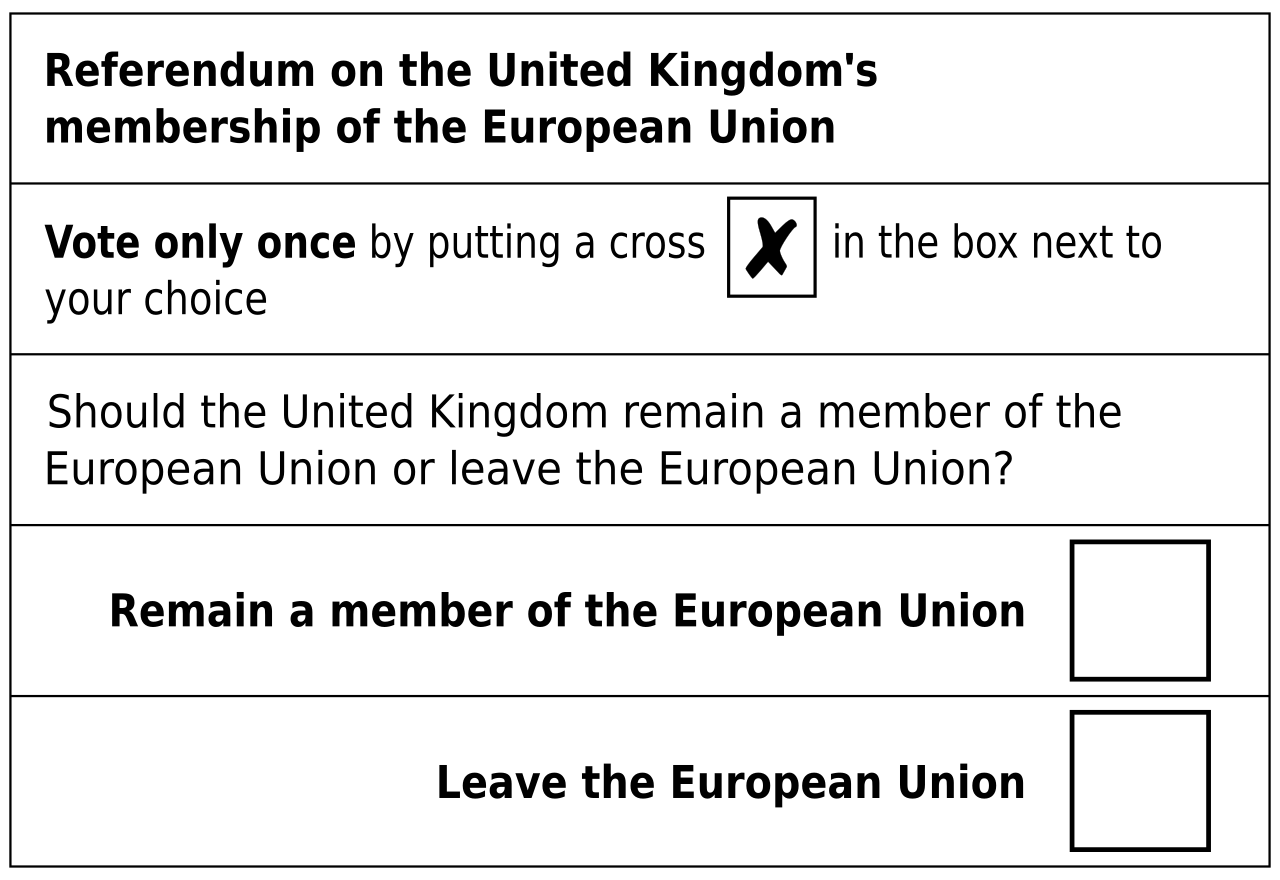
\includegraphics[width=\textwidth]{images/sample-ballot.png}
\end{center}
}

\frame{
\begin{center}
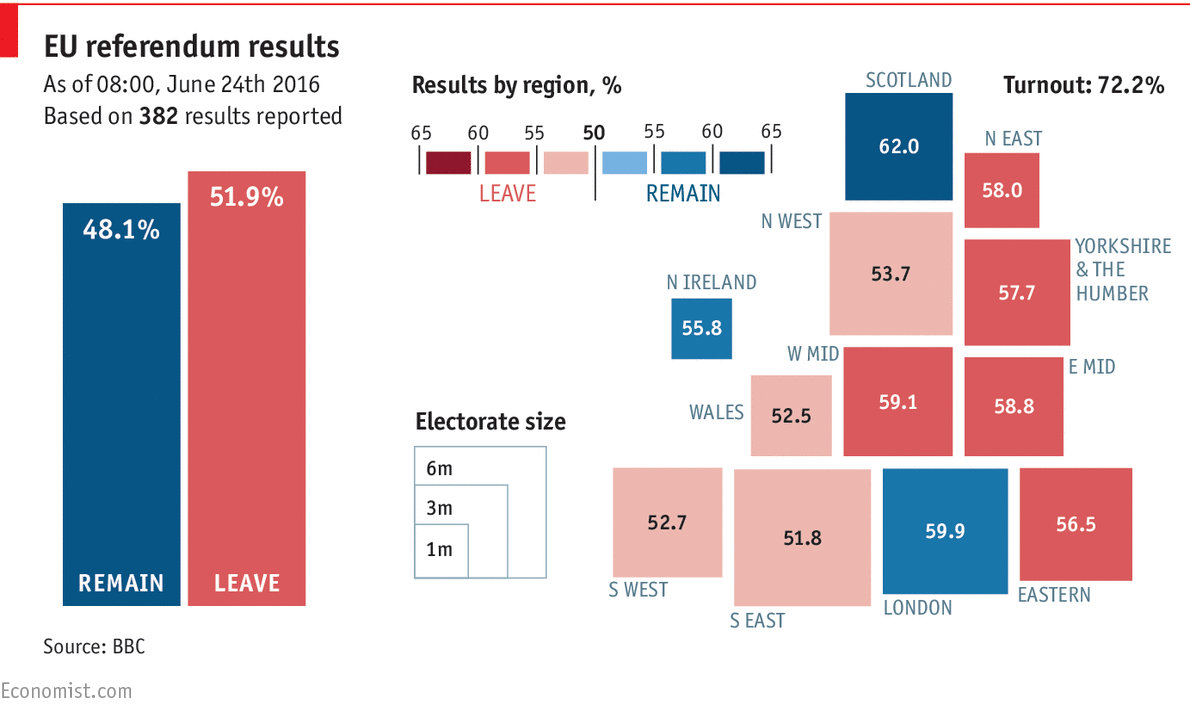
\includegraphics[width=\textwidth]{images/economist-result.png}
\end{center}
}

\frame{
\begin{center}
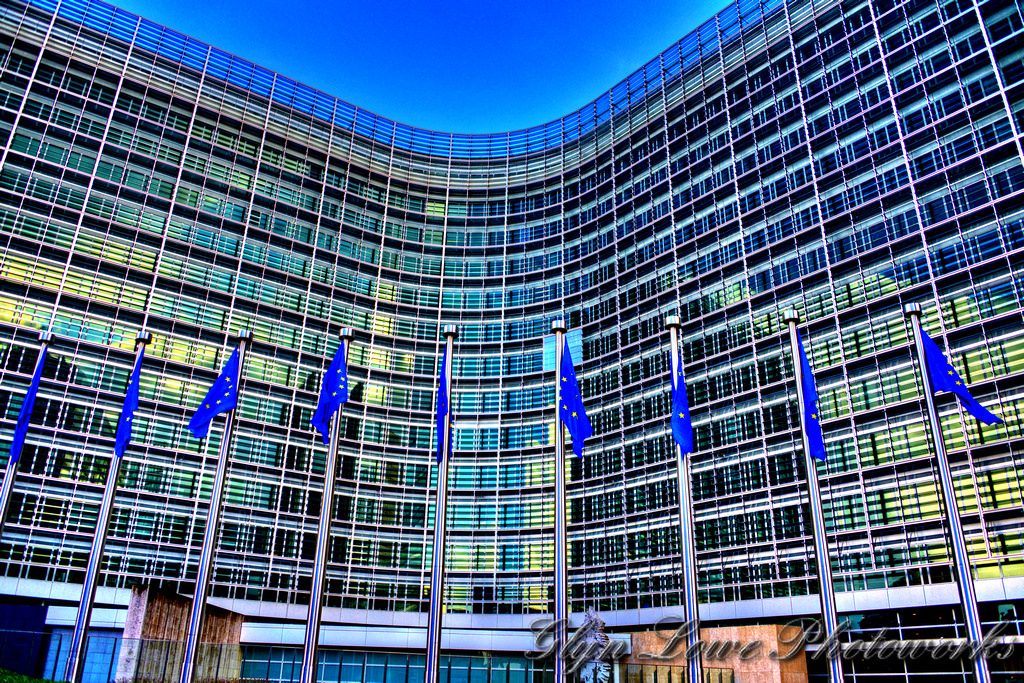
\includegraphics[height=\textheight]{images/eu-commission.png}
\end{center}
}

\frame{
\begin{center}
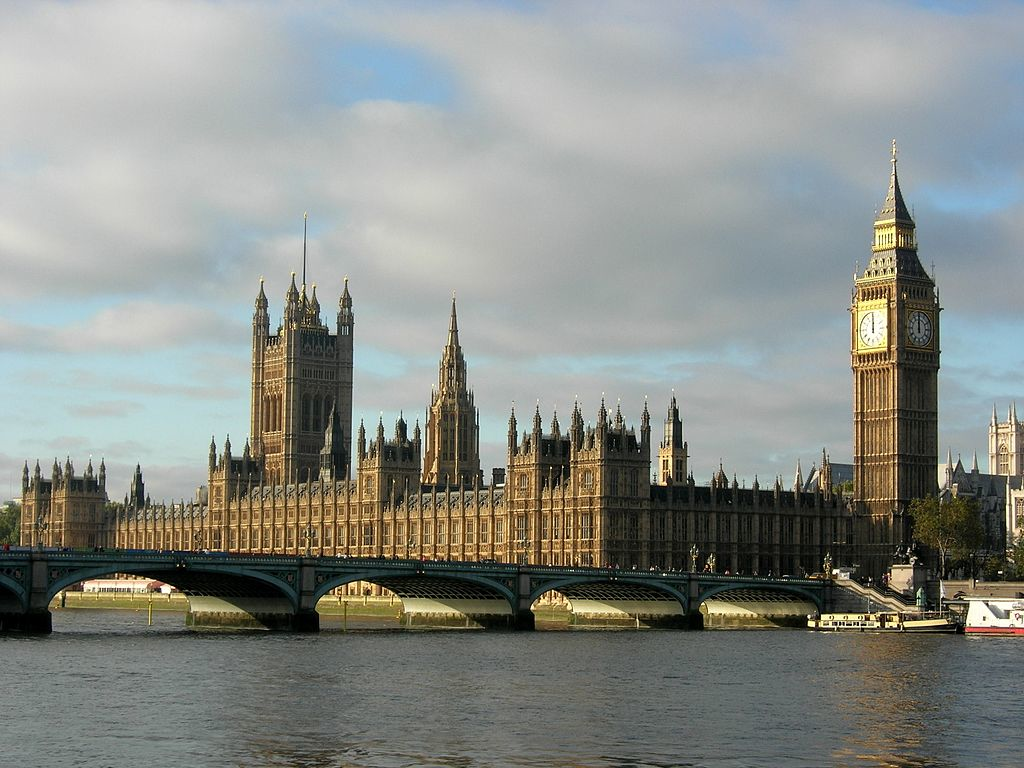
\includegraphics[height=\textheight]{images/westminster.png}
\end{center}
}


\frame{
\begin{center}
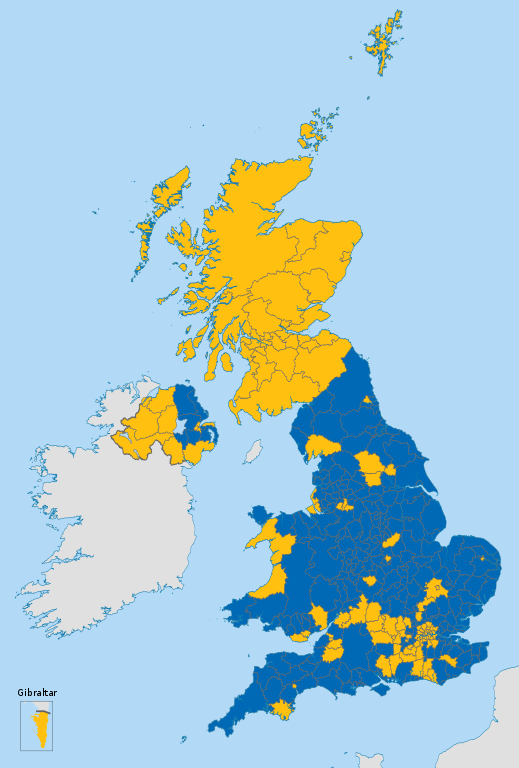
\includegraphics[height=\textheight]{images/referendum-map.png}
\end{center}
}

\frame{
\begin{center}
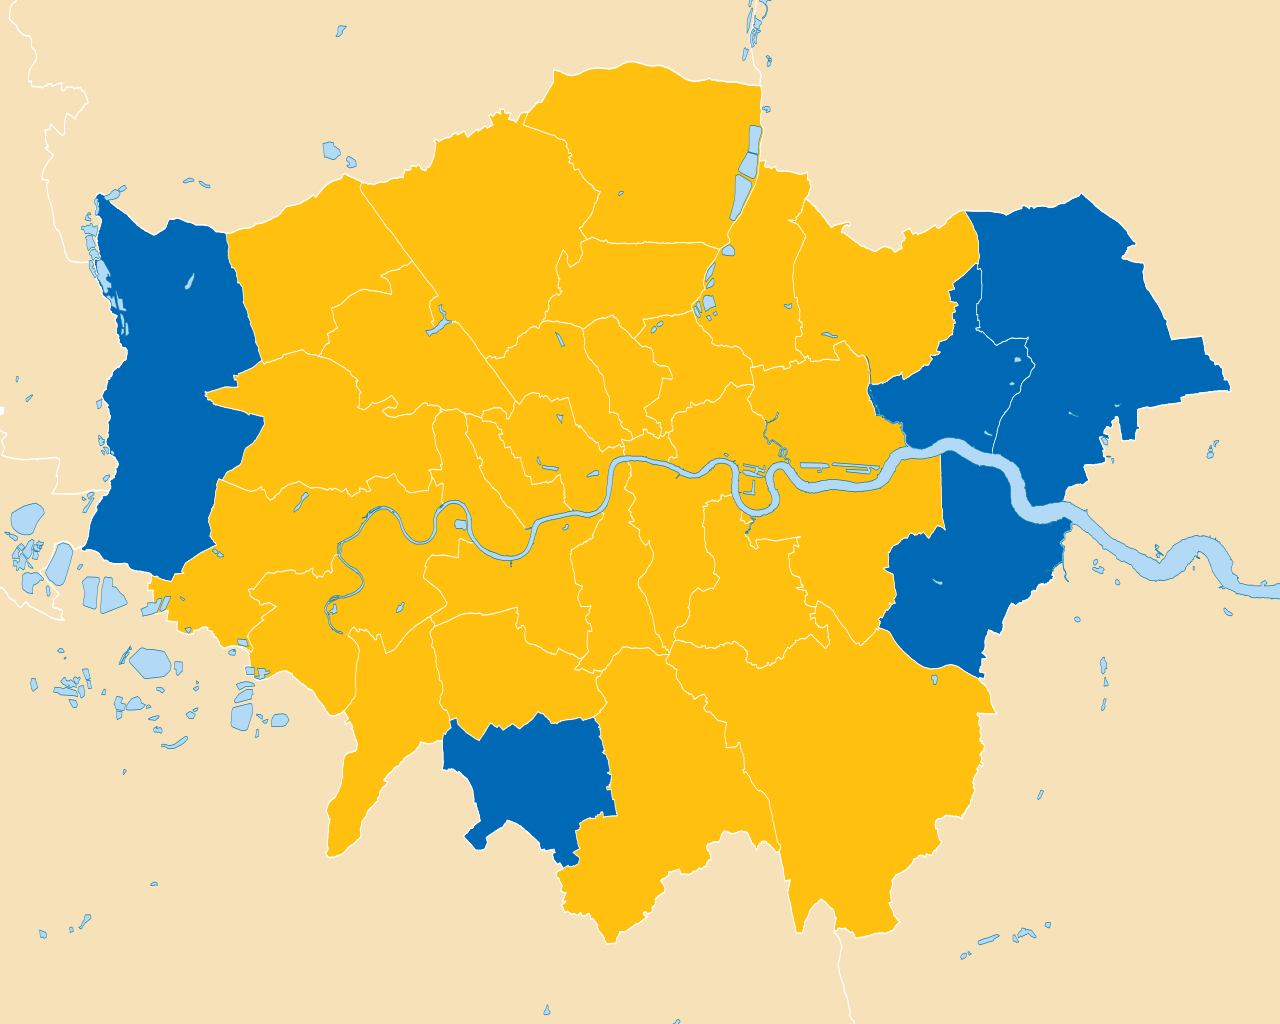
\includegraphics[height=\textheight]{images/referendum-map-london.png}
\end{center}
}


\frame{
\begin{center}
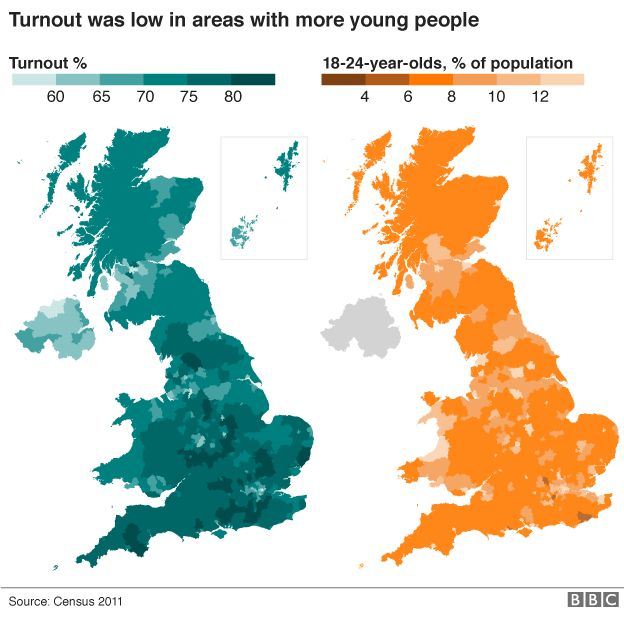
\includegraphics[height=\textheight]{images/referendum-turnout-map.png}
\end{center}
}


\frame{
\begin{center}
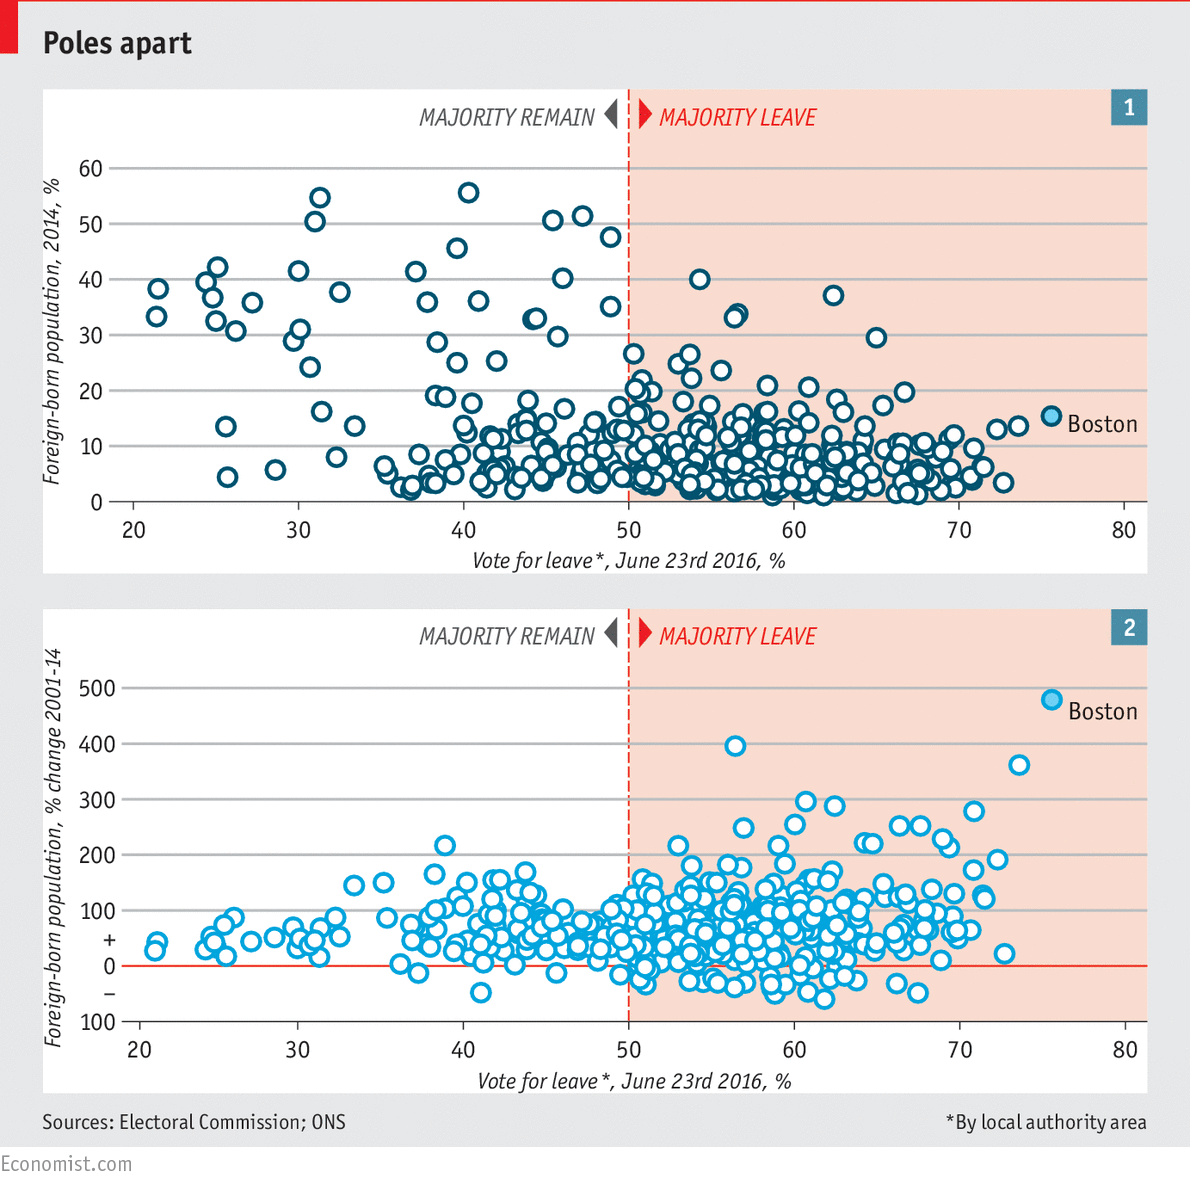
\includegraphics[height=\textheight]{images/immigration-scatterplot.png}
\end{center}
}

\frame{
\begin{center}
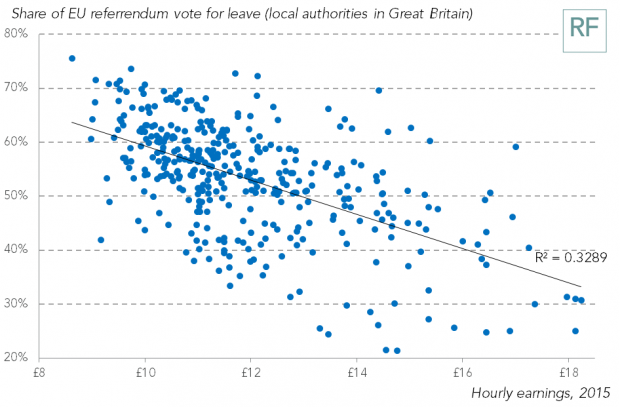
\includegraphics[width=\textwidth]{images/wages-scatterplot.png}
\end{center}
}

\frame{
\begin{center}
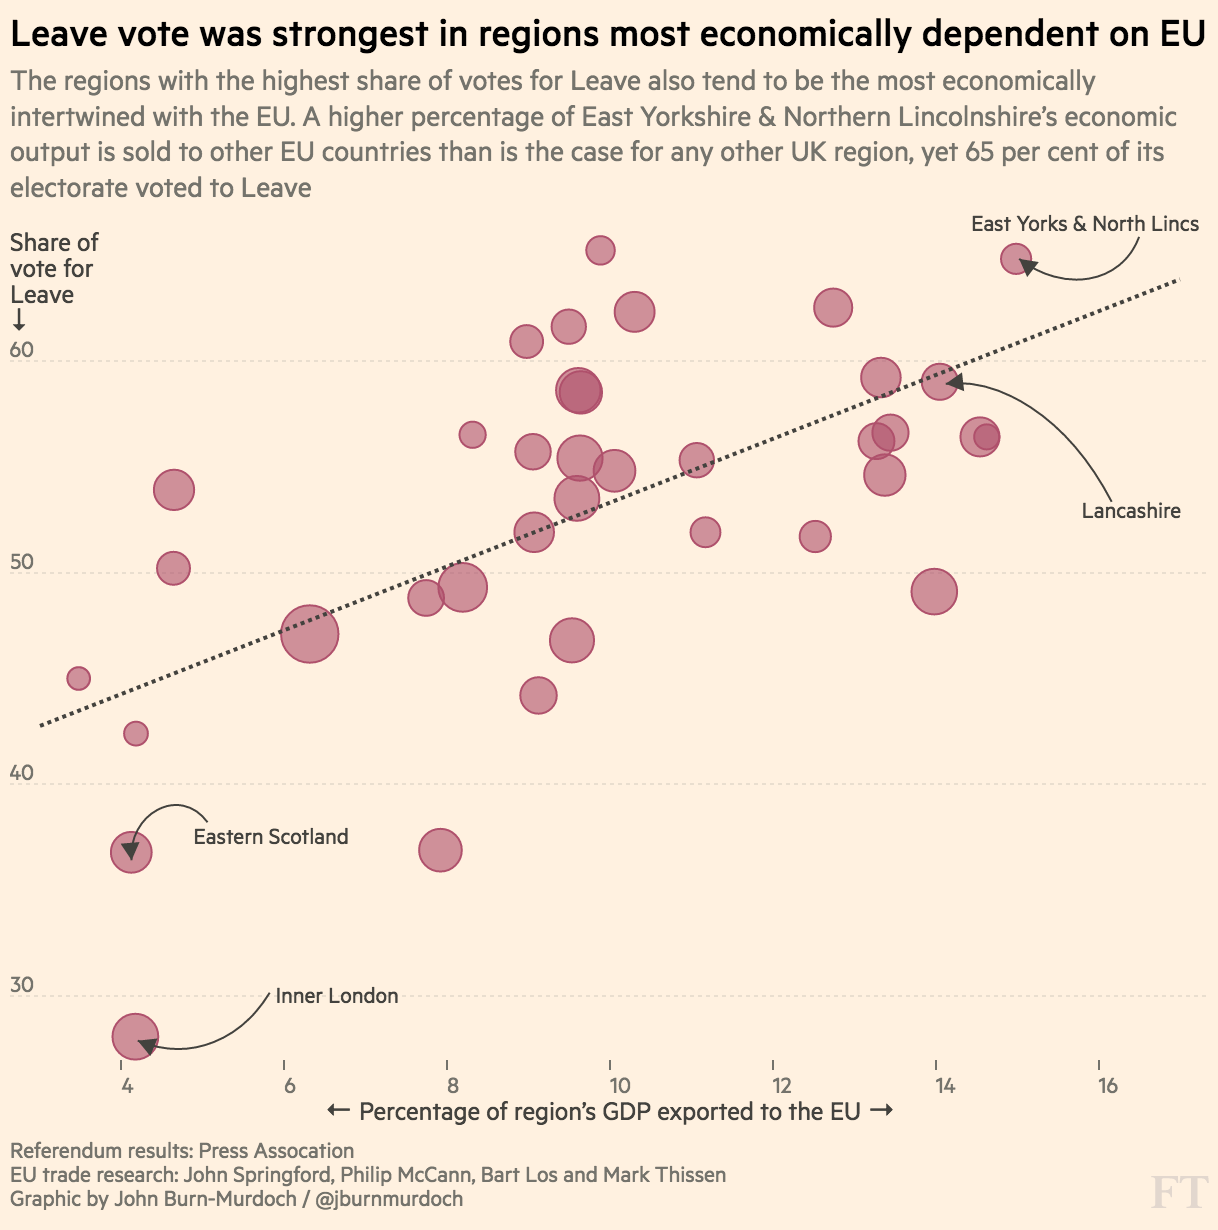
\includegraphics[height=\textheight]{images/brexit-exports-scatterplot.png}
\end{center}
}

\frame{
\begin{center}
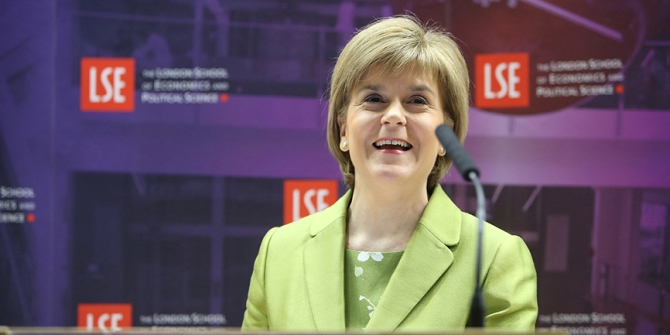
\includegraphics[width=\textwidth]{images/nicola-sturgeon.png}
\end{center}
}

\frame{
\begin{center}
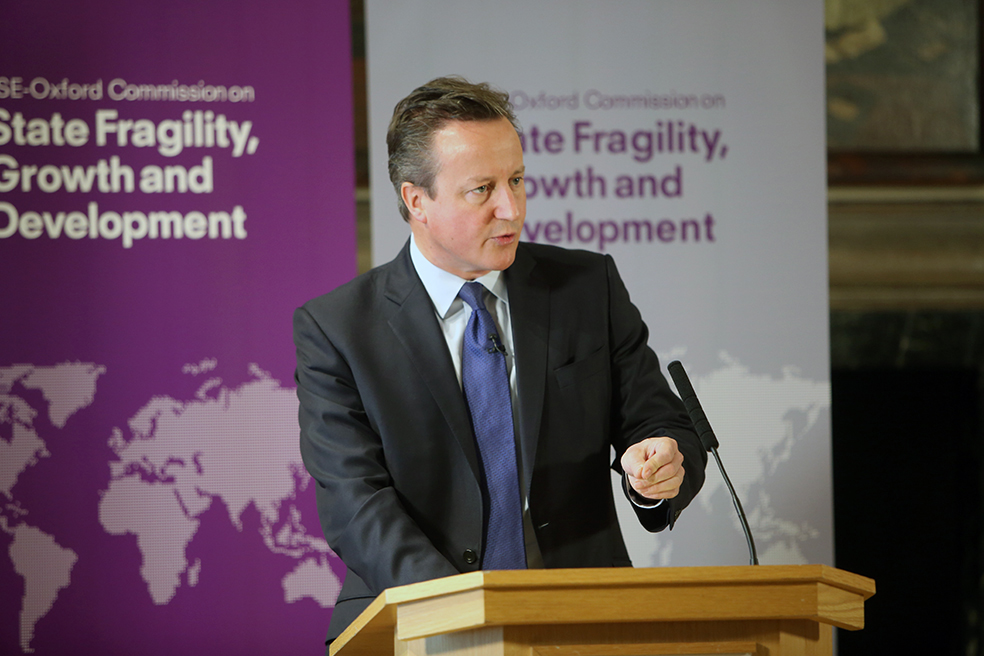
\includegraphics[width=\textwidth]{images/david-cameron.png}
\end{center}
}

\frame{
\begin{center}
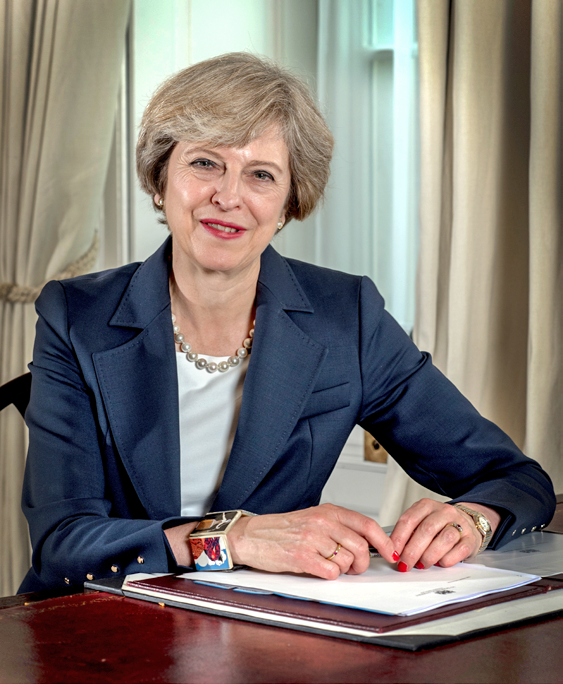
\includegraphics[height=\textheight]{images/theresa-may.png}
\end{center}
}

\frame{
\begin{center}
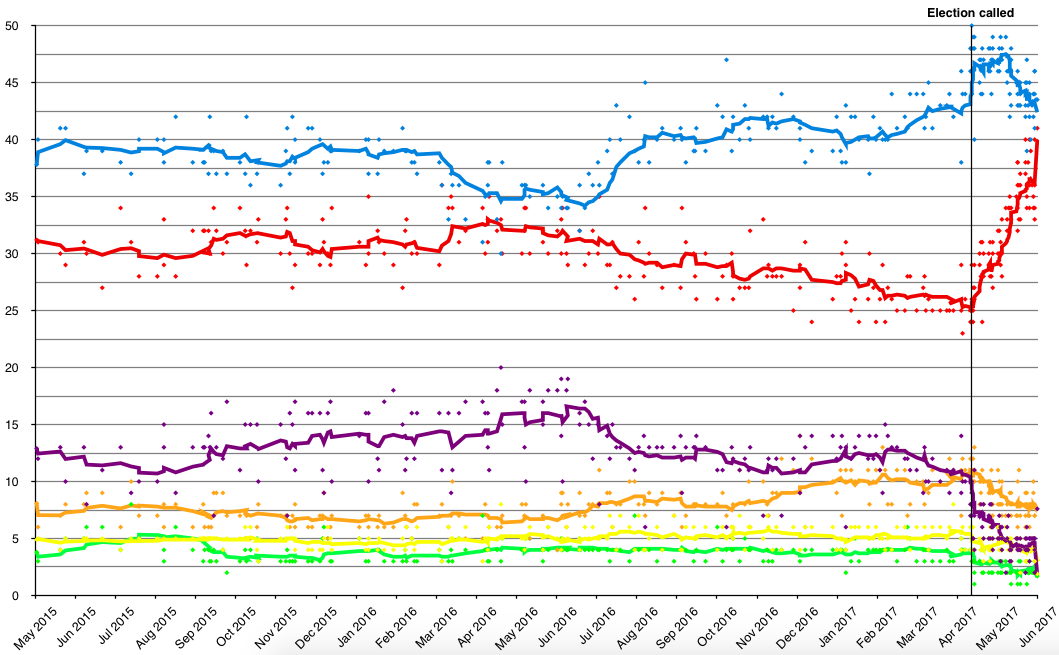
\includegraphics[width=\textwidth]{images/ge2017-poll-trend.png}
\end{center}
}

\frame{
\begin{center}
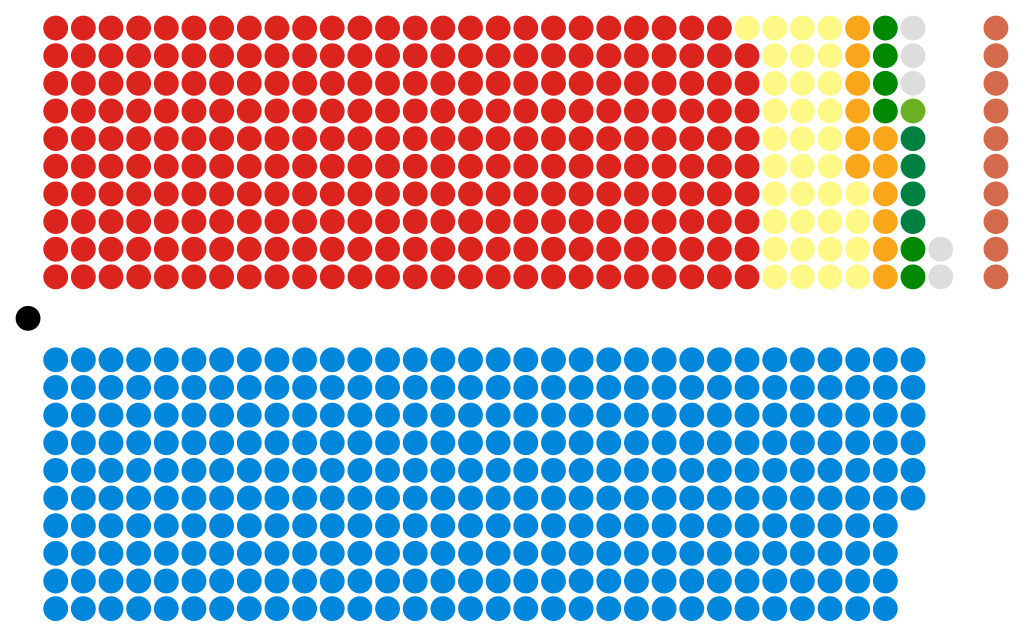
\includegraphics[width=\textwidth]{images/ge2017-hoc-membership.png}
\end{center}
}


\section{What Now?}
\frame{\tableofcontents[currentsection]}

\frame{
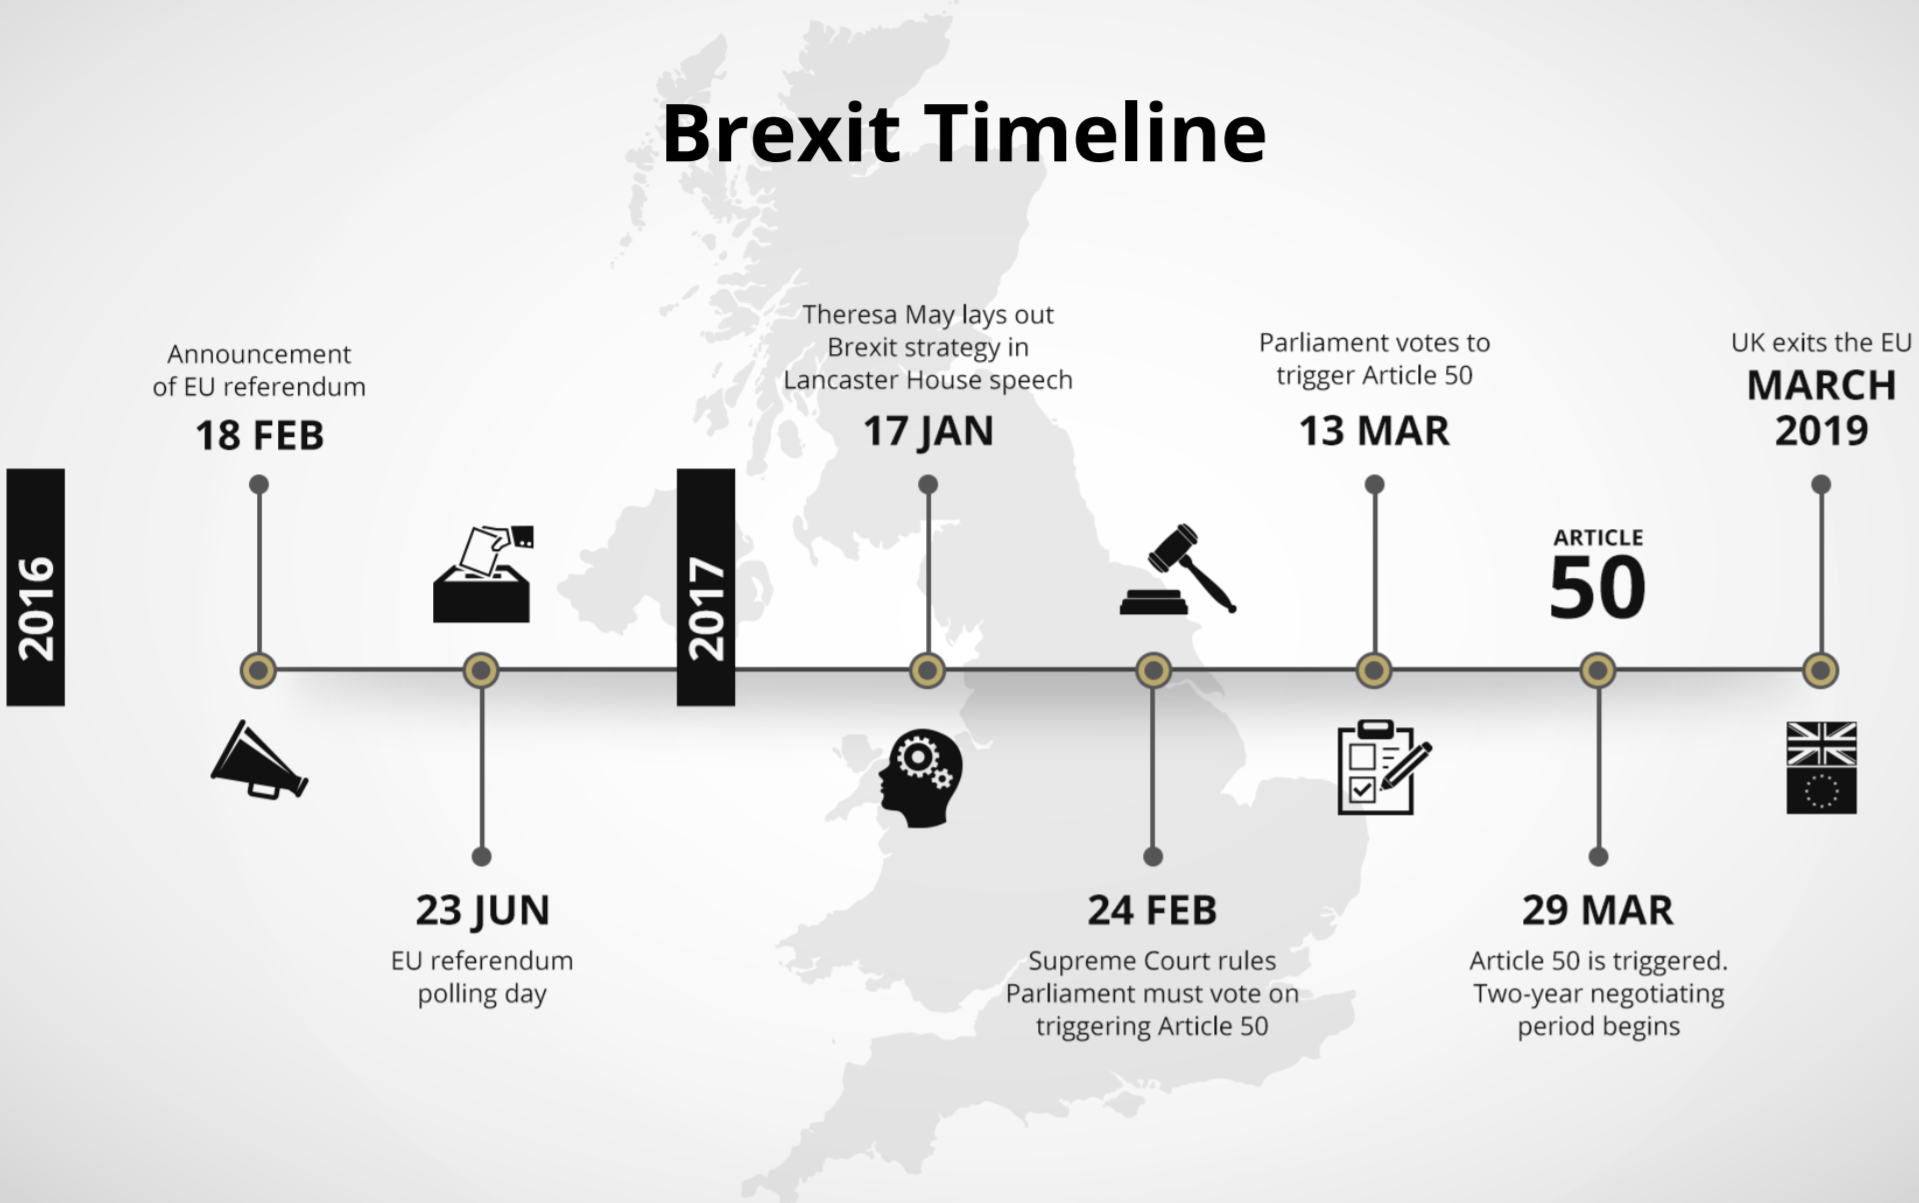
\includegraphics[width=\textwidth]{images/brexit-timeline.png}
}

\frame{

\frametitle{Summarising Trends in One Word}

\Huge
\begin{center}
\onslide<2->{Stability!}
\end{center}
}

\frame{
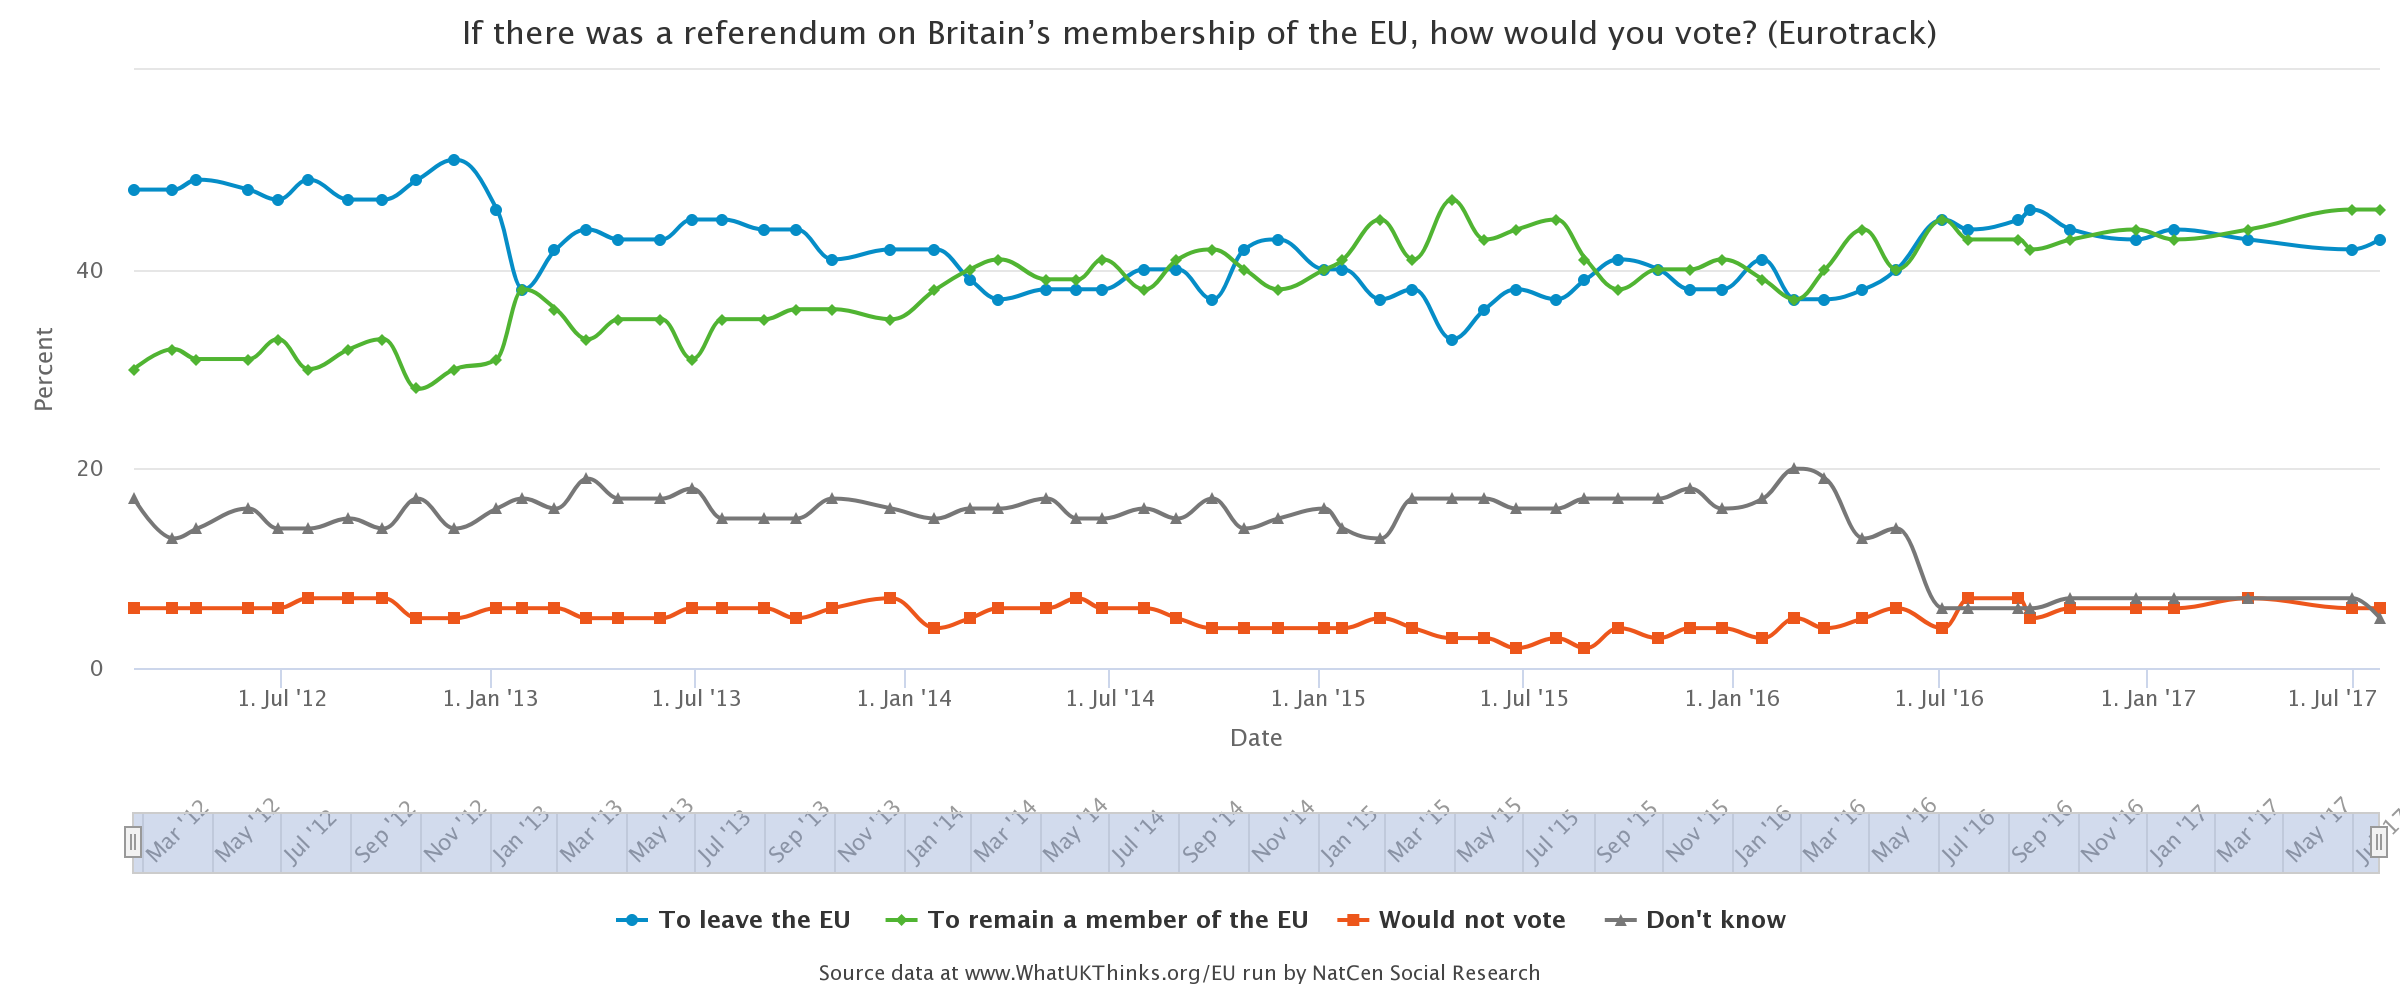
\includegraphics[width=\textwidth]{images/how-would-you-vote.png}
\vspace{1em}
\footnotesize{Source: NatCen Social Research (What UK Thinks)}
}


\frame{
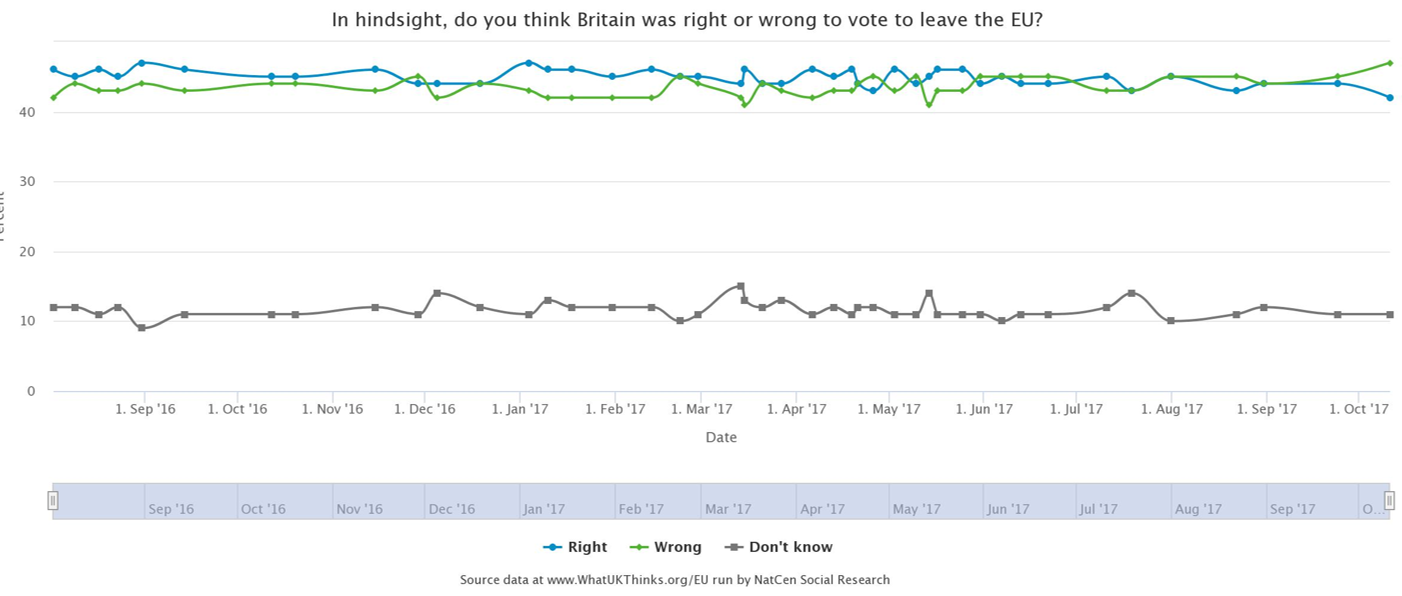
\includegraphics[width=\textwidth]{images/right-wrong.png}
\vspace{1em}
\footnotesize{Source: NatCen Social Research (What UK Thinks)}
}

\frame{Stability! Except\dots}

\frame{
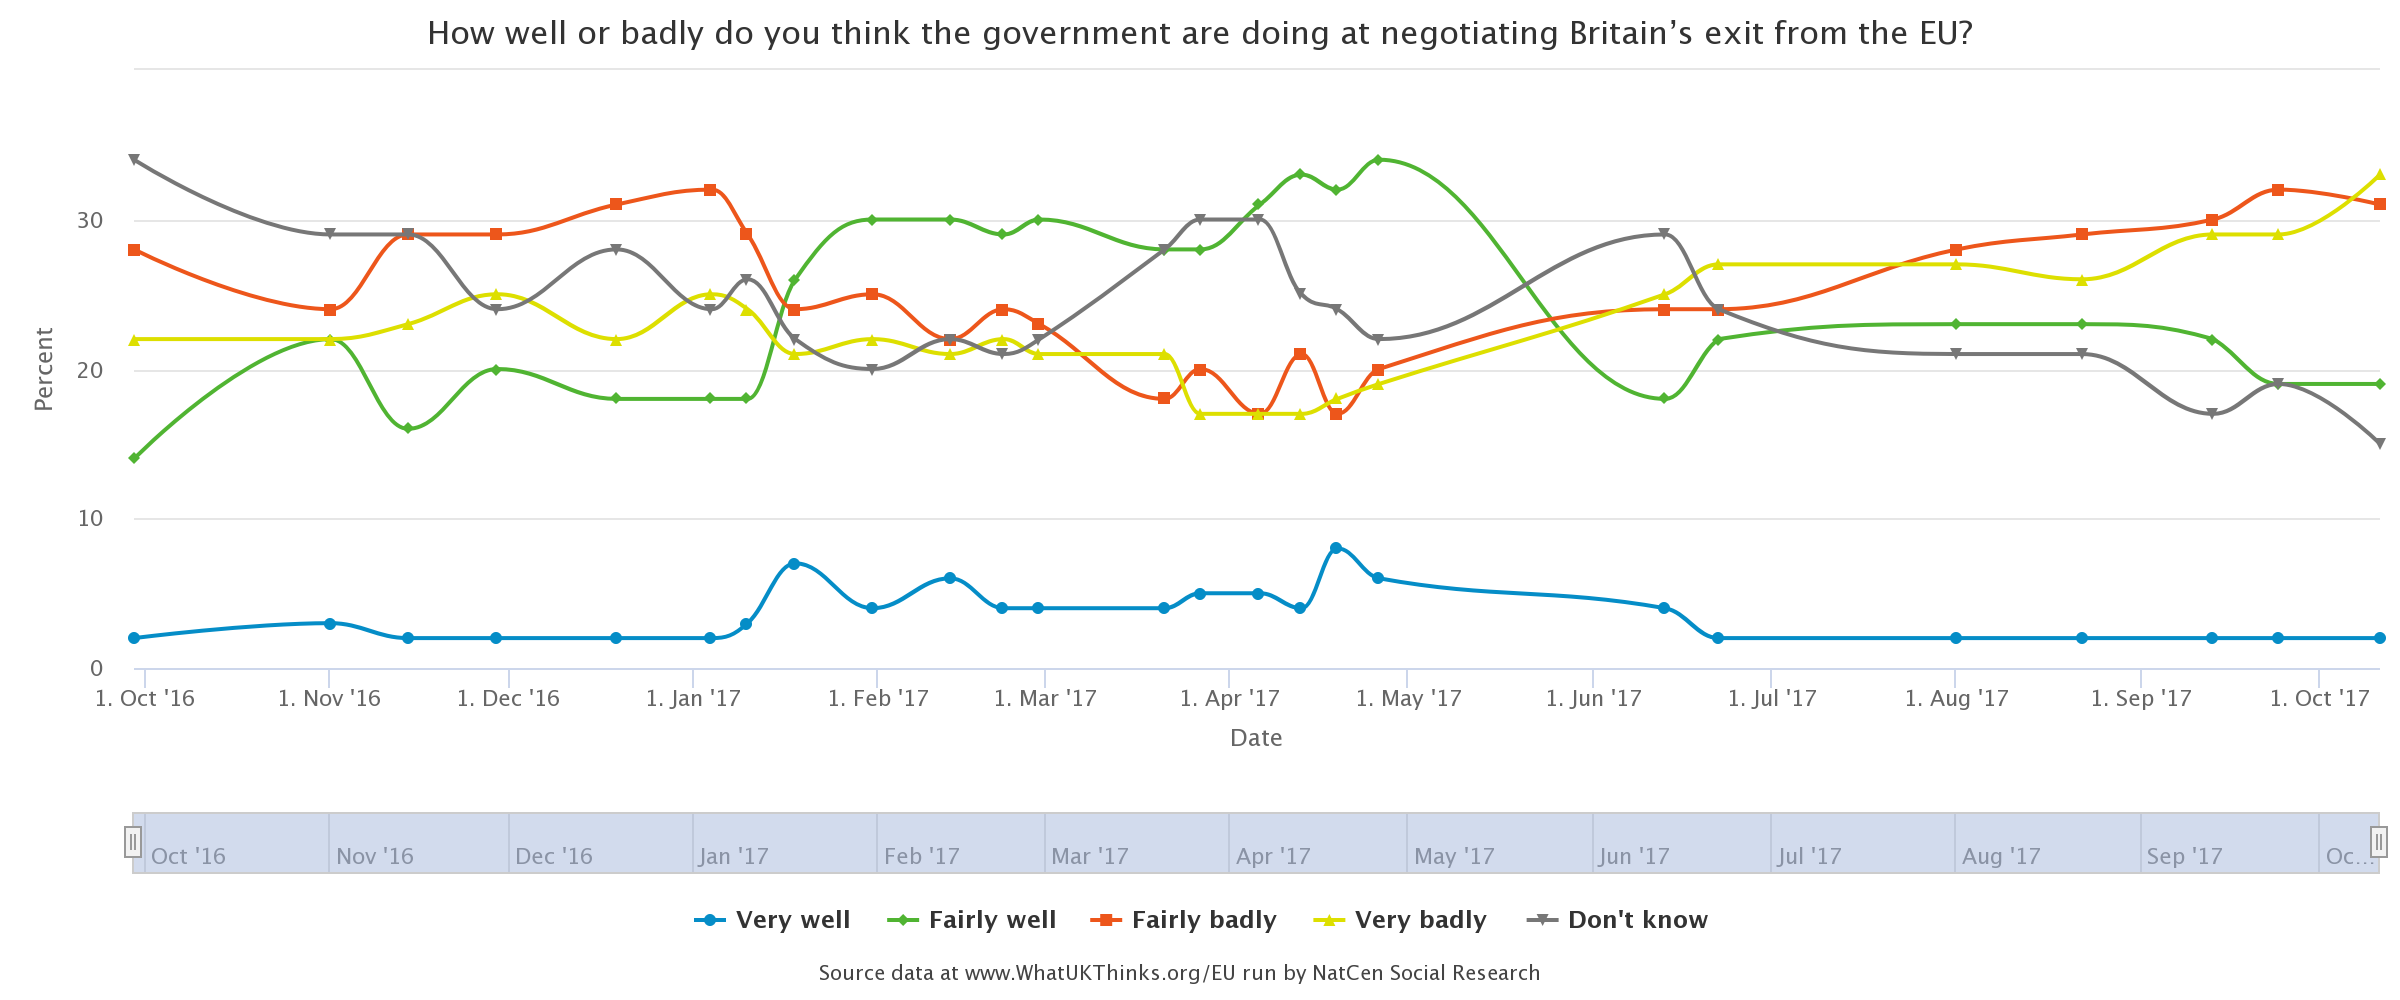
\includegraphics[width=\textwidth]{images/government-performance.png}
\vspace{1em}
\footnotesize{Source: NatCen Social Research (What UK Thinks)}
}

\frame{
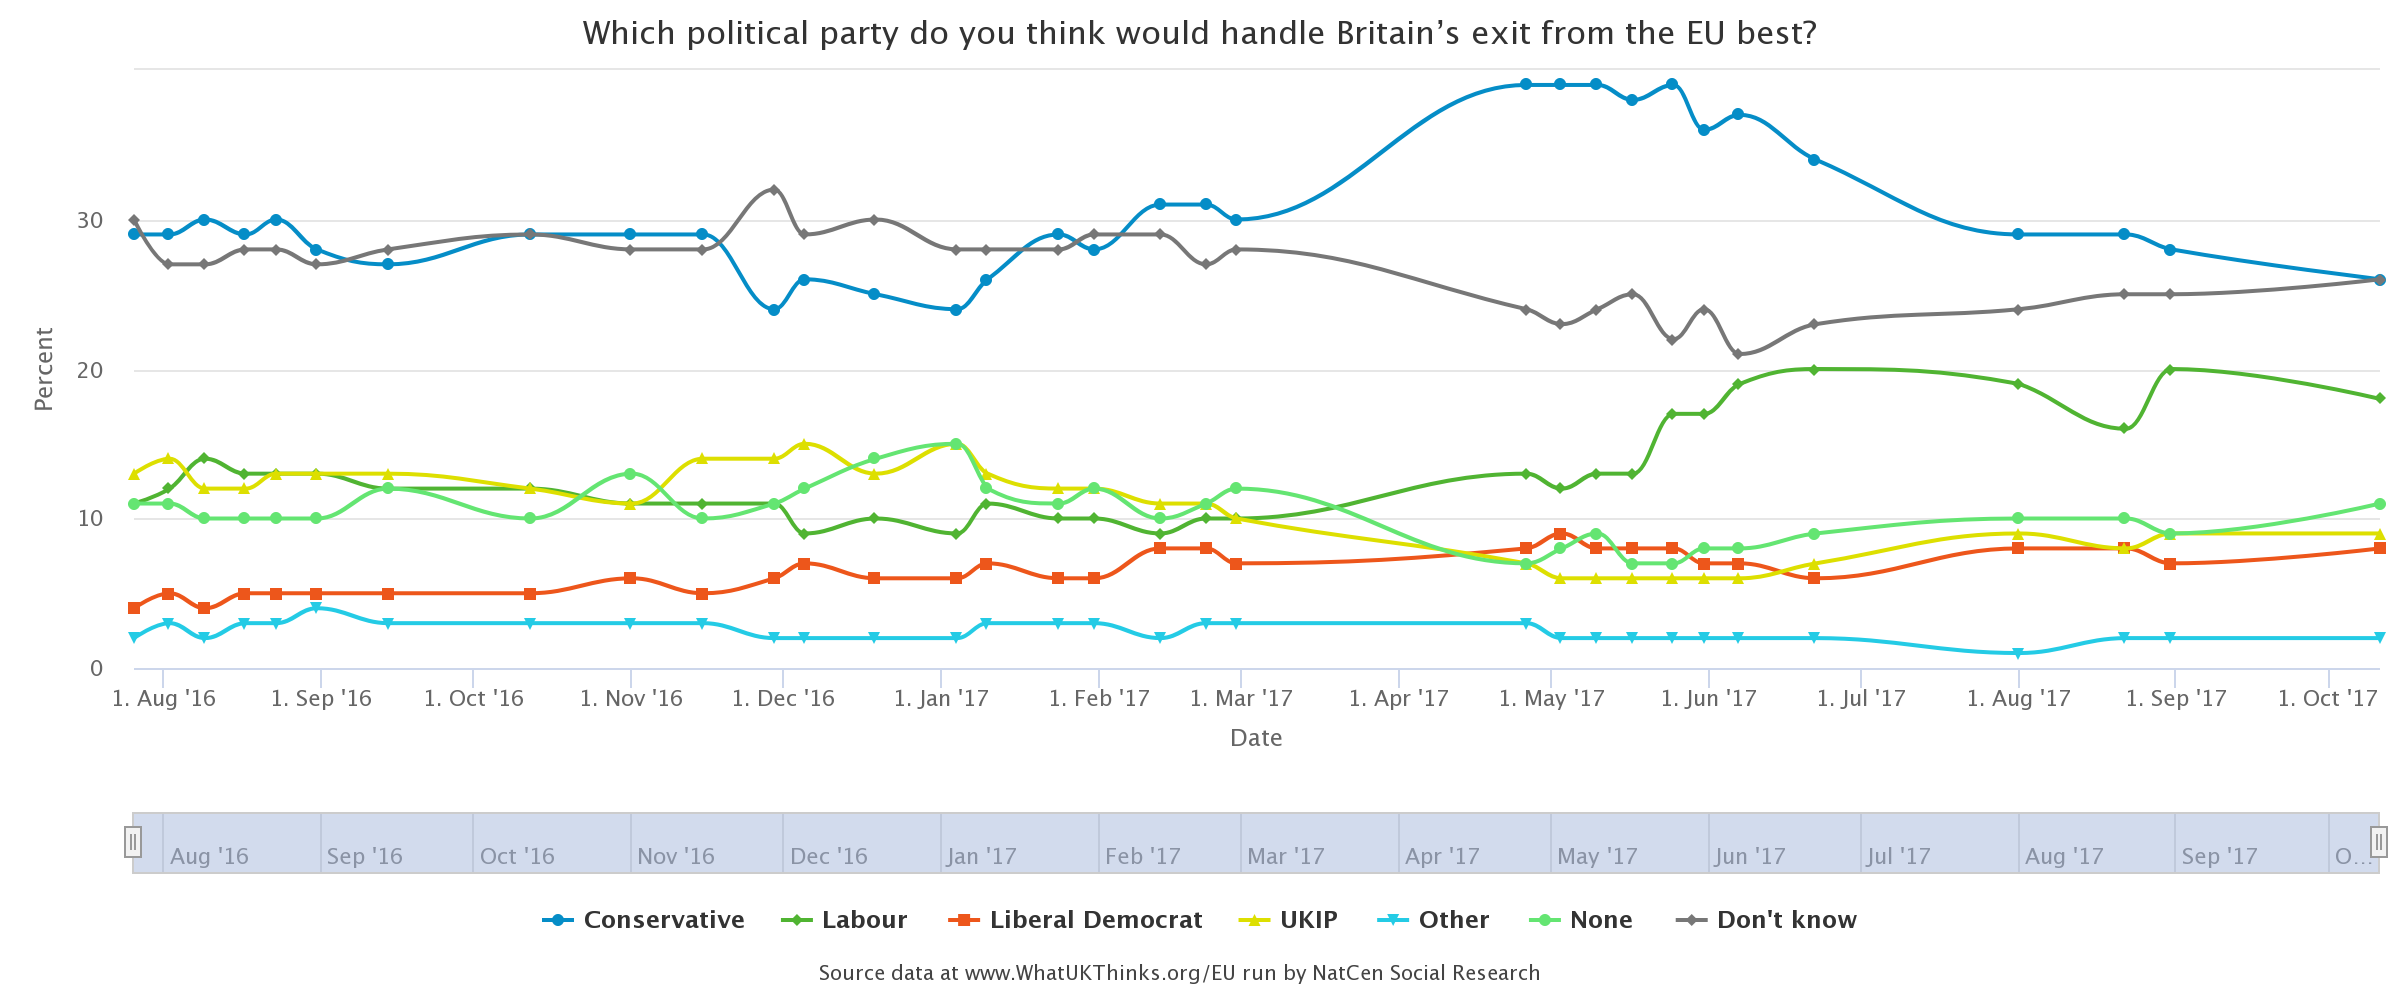
\includegraphics[width=\textwidth]{images/best-party.png}
\vspace{1em}
\footnotesize{Source: NatCen Social Research (What UK Thinks)}
}

\frame{
\frametitle{What do voters want?}
\begin{center}
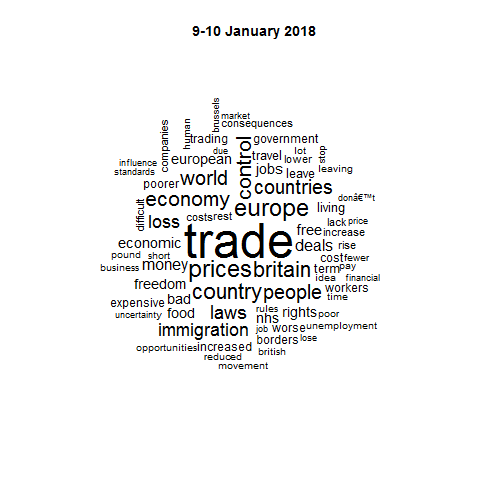
\includegraphics[height=\textheight]{images/wordcloud4-all}
\end{center}
\hltfootnote
}

\frame{

\frametitle{What do voters want?}

\begin{enumerate}
\item Immigration/freedom of movement
\item Jurisdiction of the ECJ
\item Rights of EU (UK) citizens in UK (EU)
\item `Divorce bill'
\item Ongoing payments to EU budget
\item Trade agreement
\item Northern Ireland border
\item Timeline for implementation
\end{enumerate}

}

\frame{
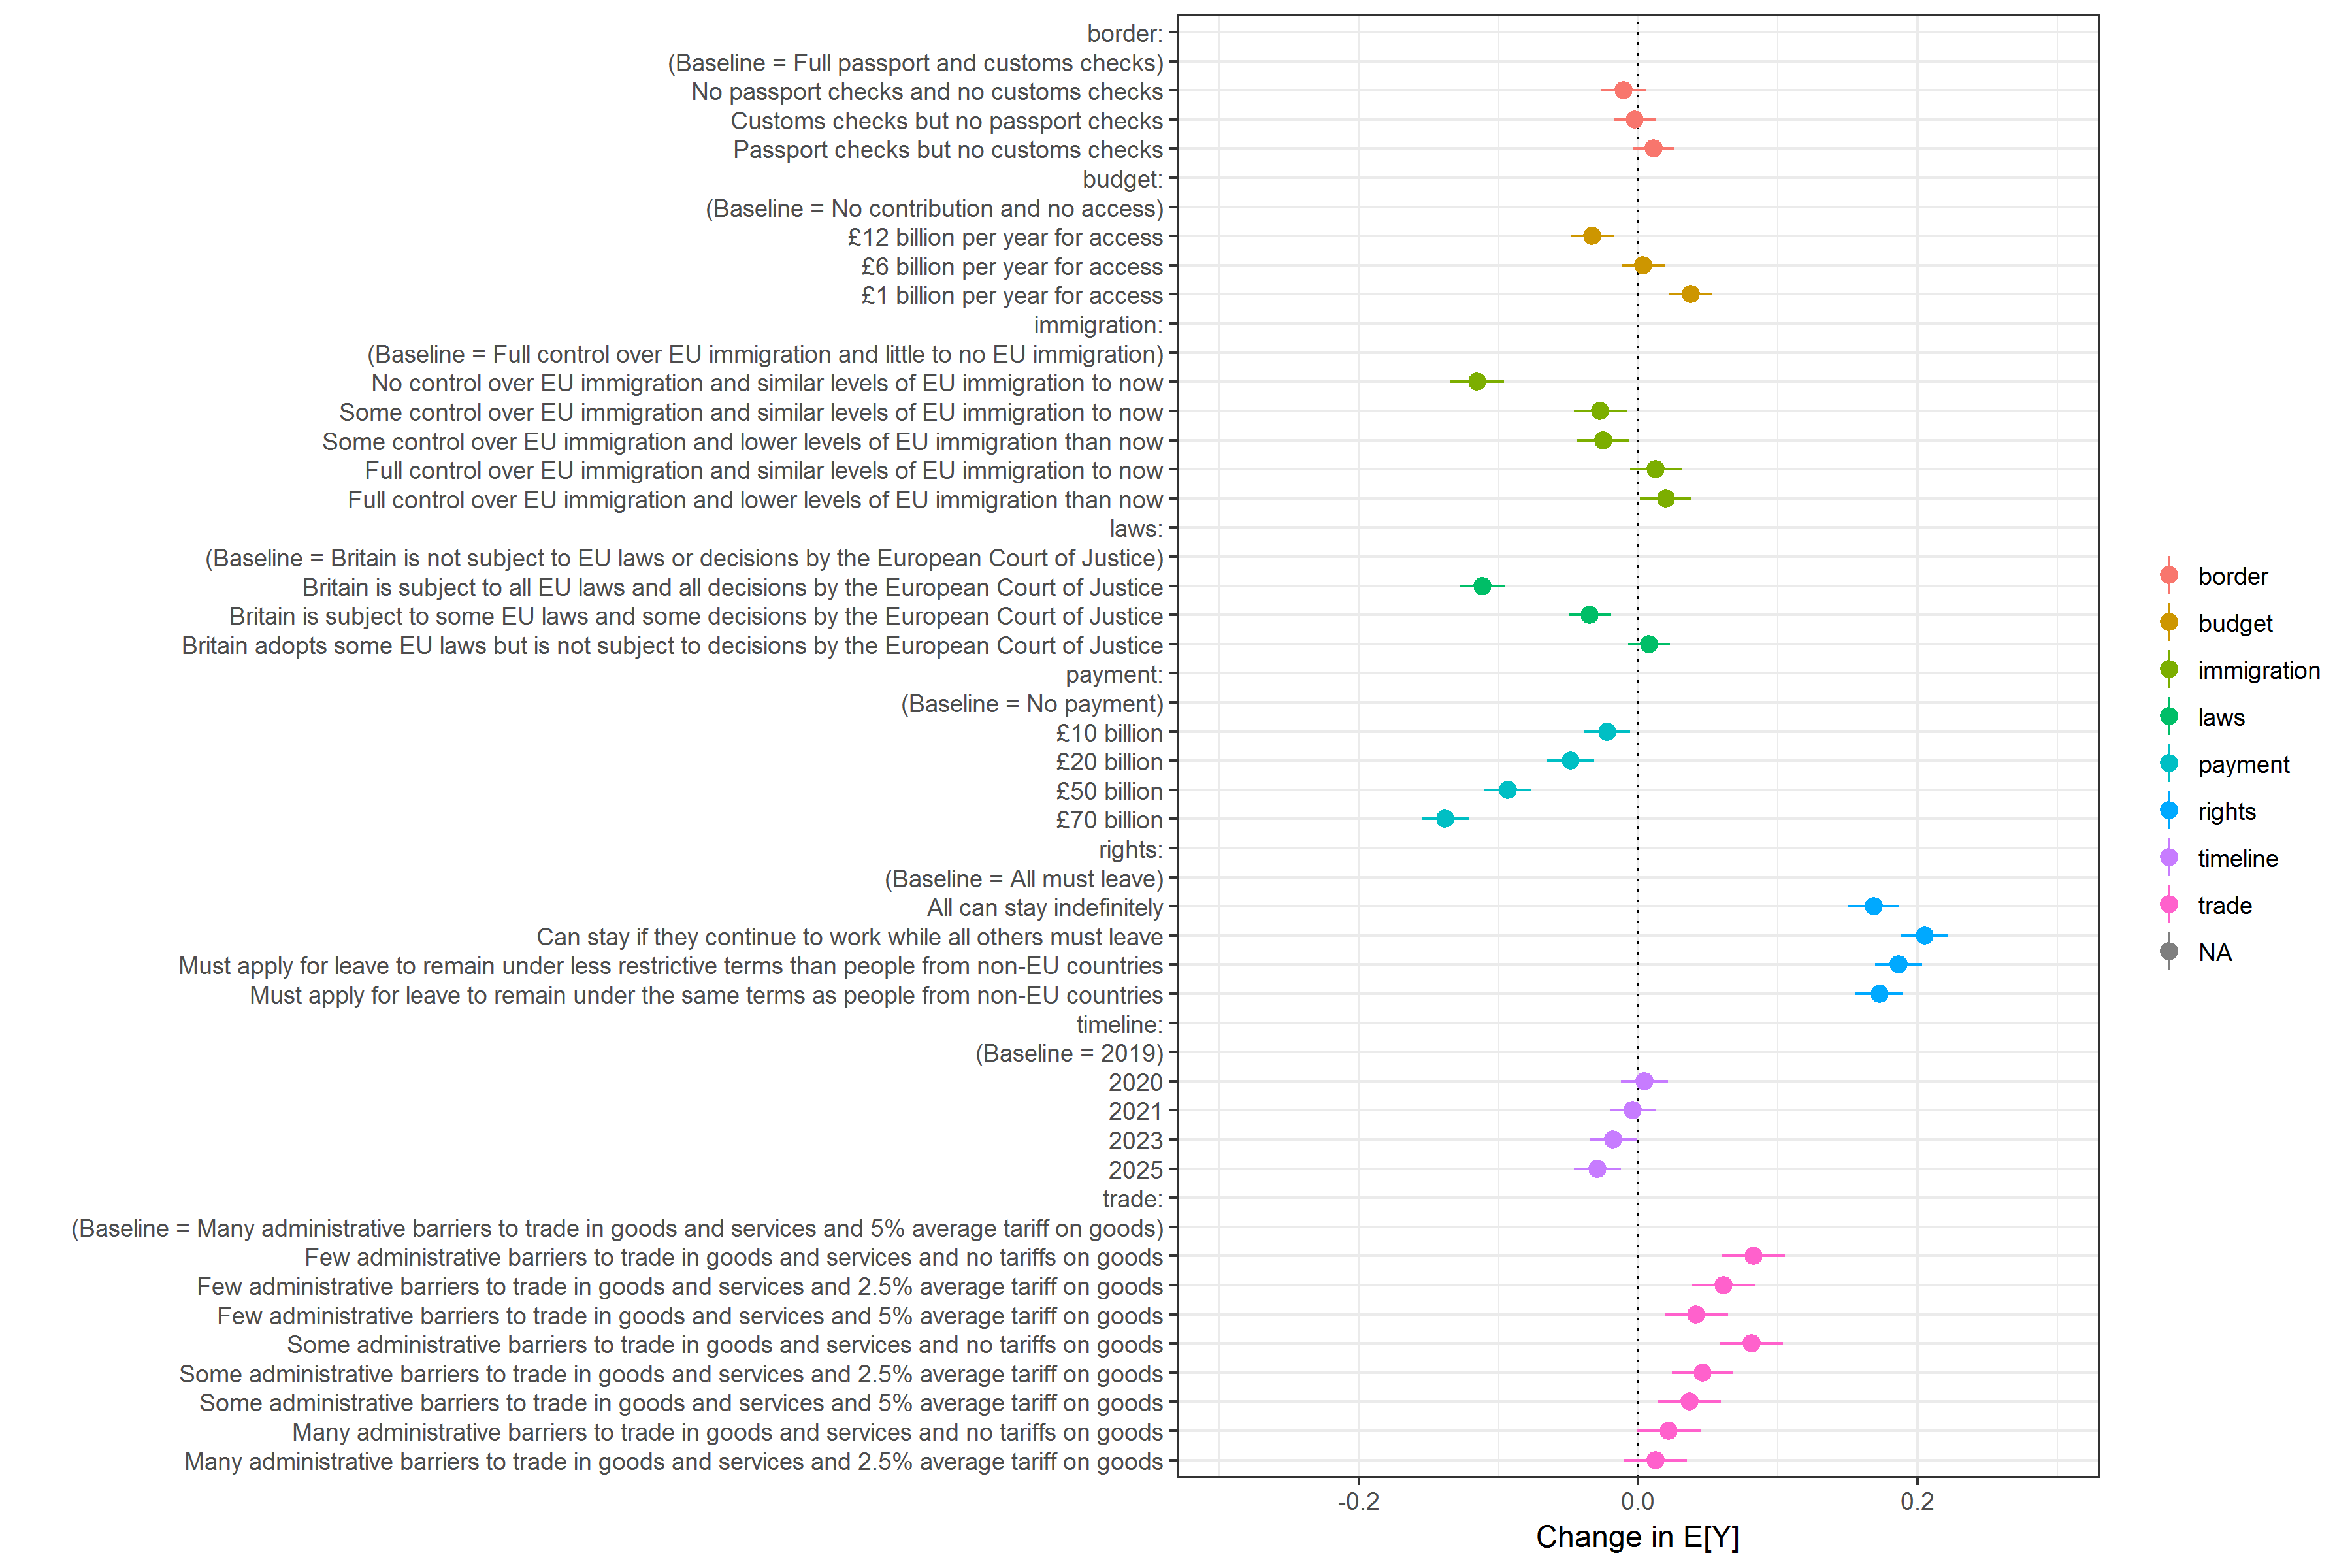
\includegraphics[height=\textheight]{images/amceQ1.png}
\hltfootnote
}

\frame{
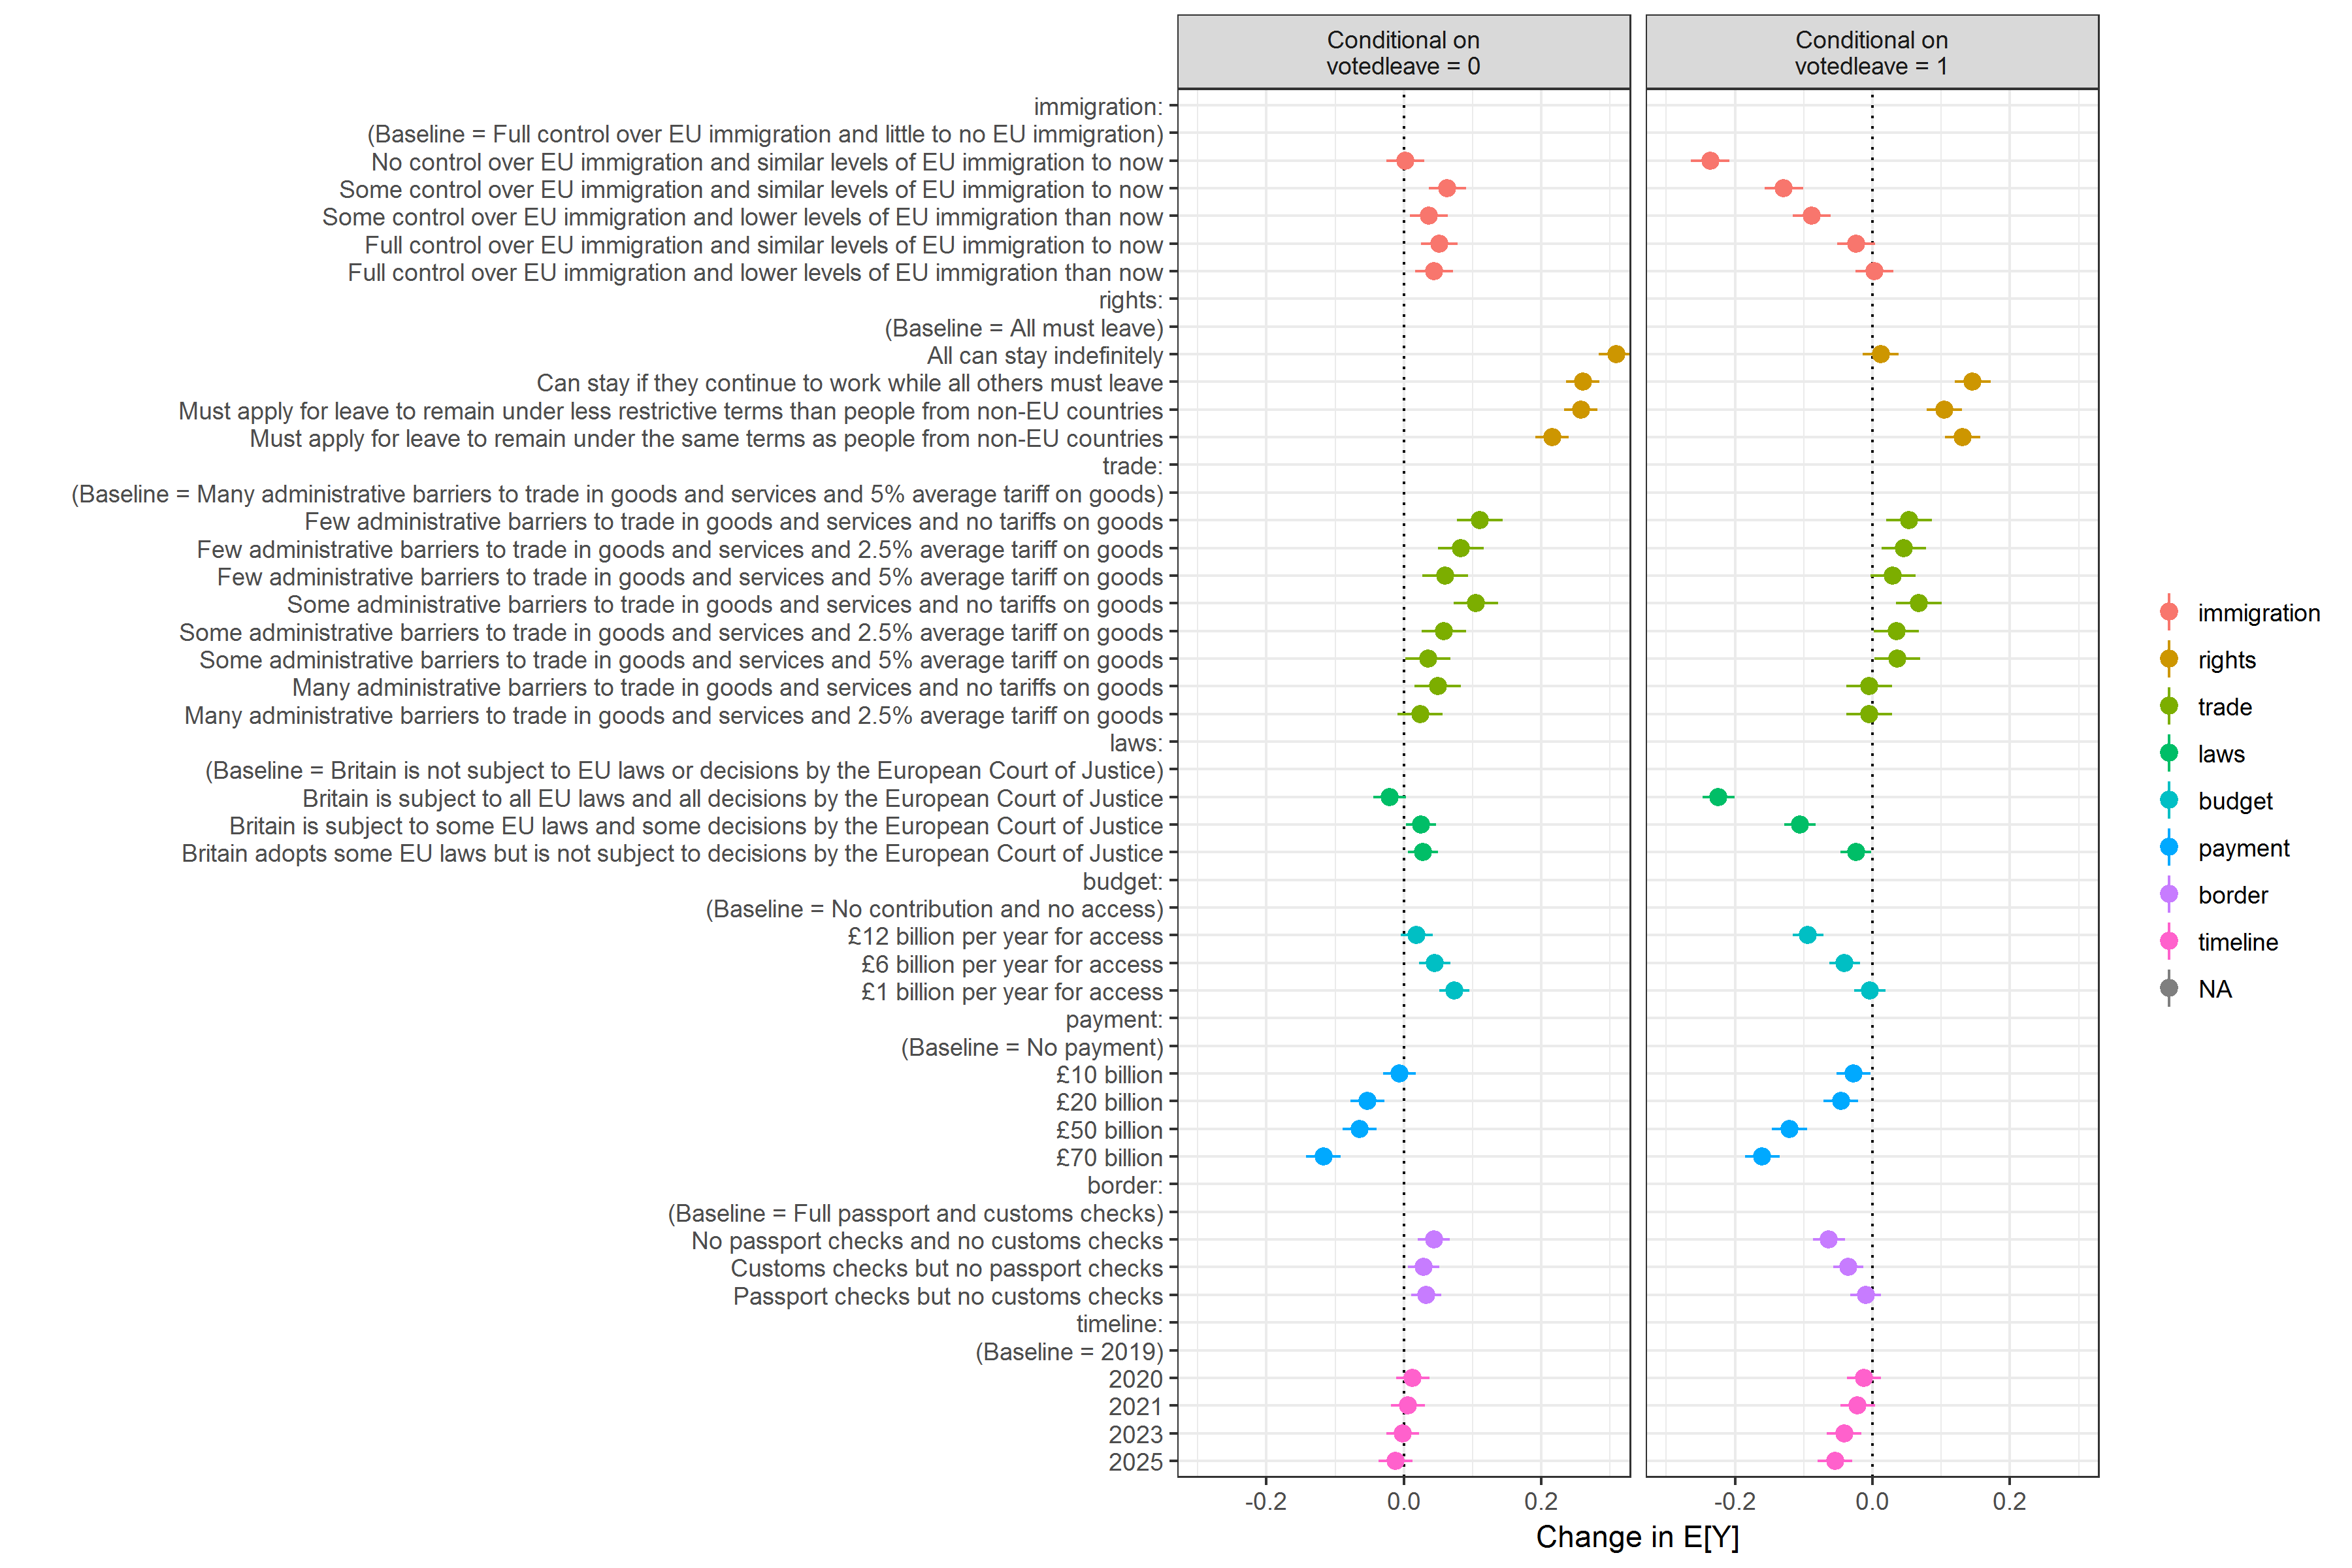
\includegraphics[height=\textheight]{images/amceQ1_byvote.png}
\hltfootnote
}


\frame{}

\frame{
\begin{center}
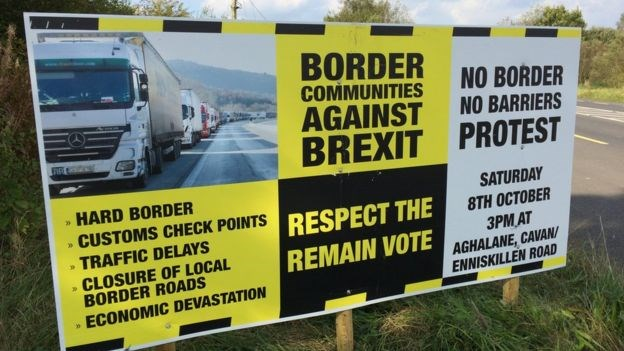
\includegraphics[width=\textwidth]{images/northern-ireland-border.png}
\end{center}
}

\frame{
\begin{center}
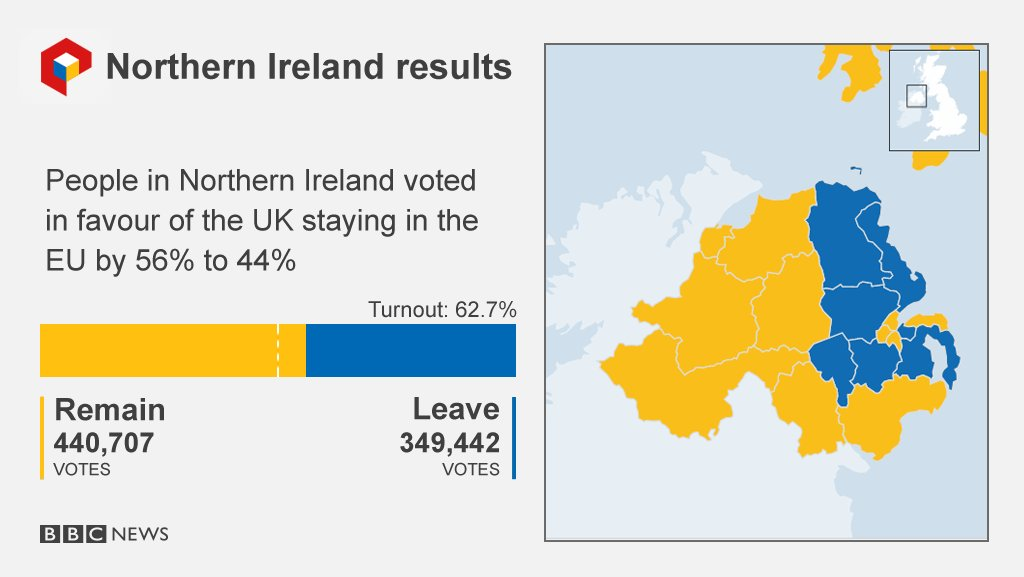
\includegraphics[width=\textwidth]{images/results-northern-ireland.png}
\end{center}
}



\frame{}

\frame{
\frametitle{Perceived Effects of Brexit}
\textit{Do you think leaving the European Union will have a positive or negative effect \textbf{on Britain}?}

\begin{center}
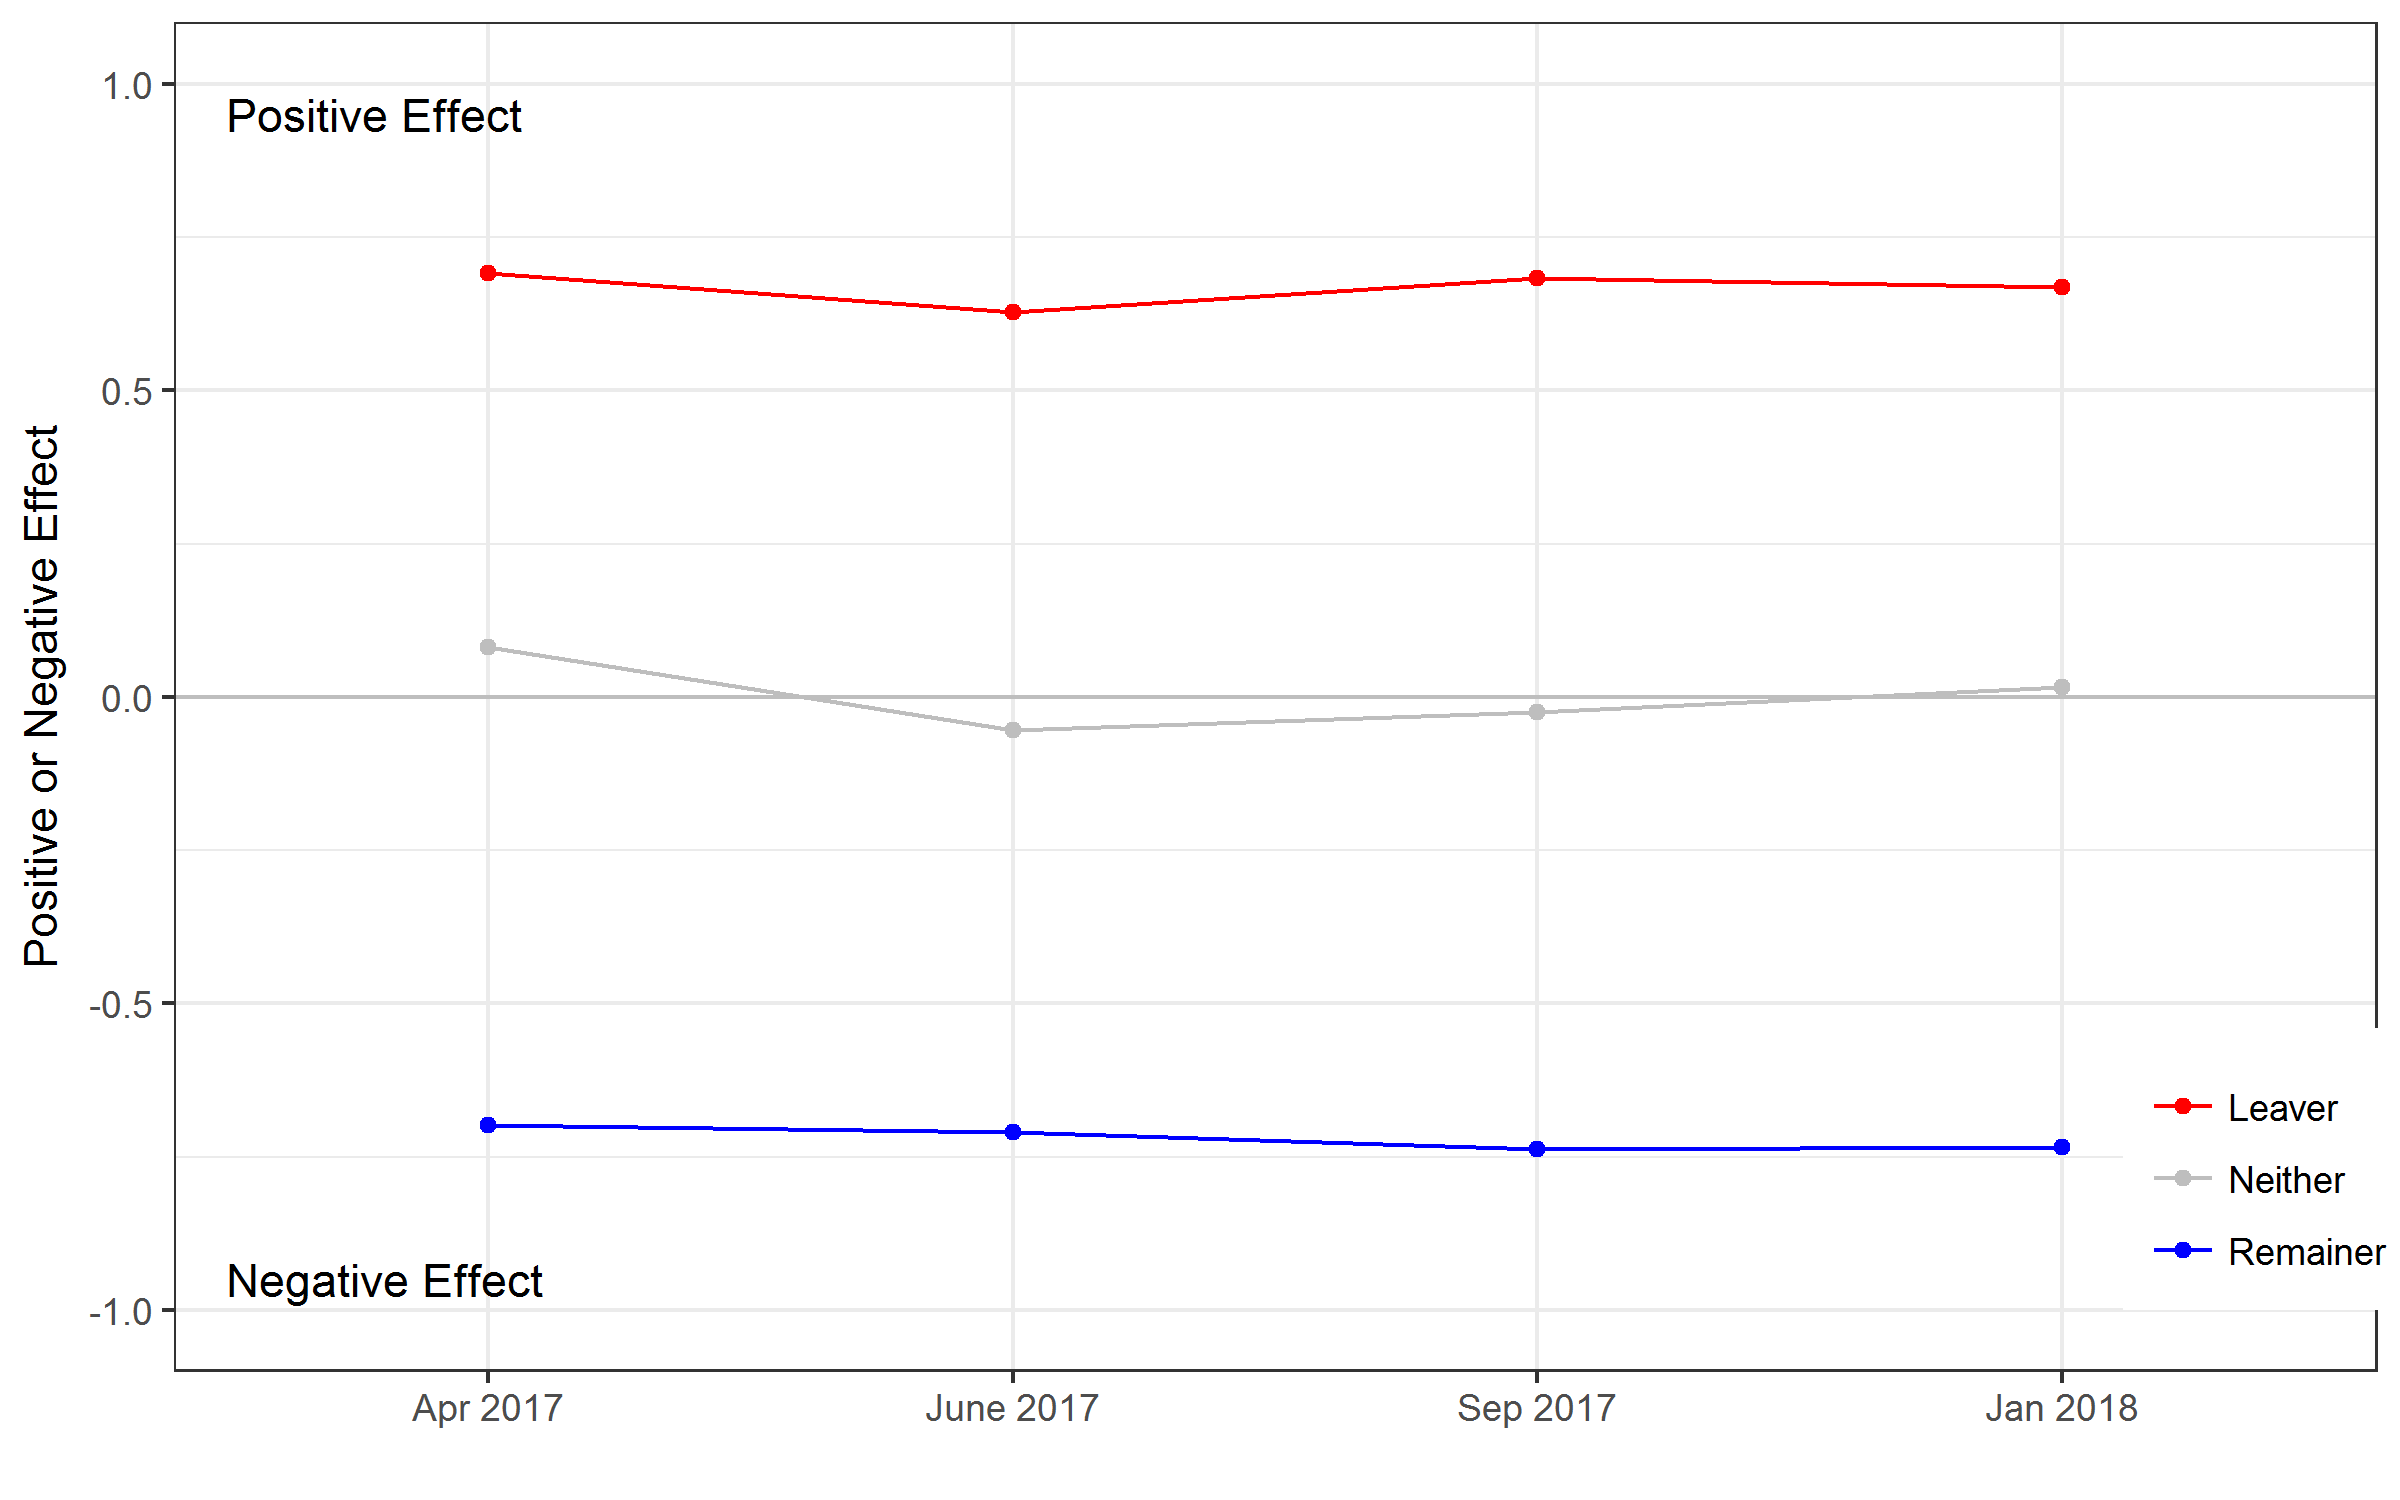
\includegraphics[width=.8\textwidth]{images/trend-effectuk.png}
\end{center}
}


\frame{
\begin{center}
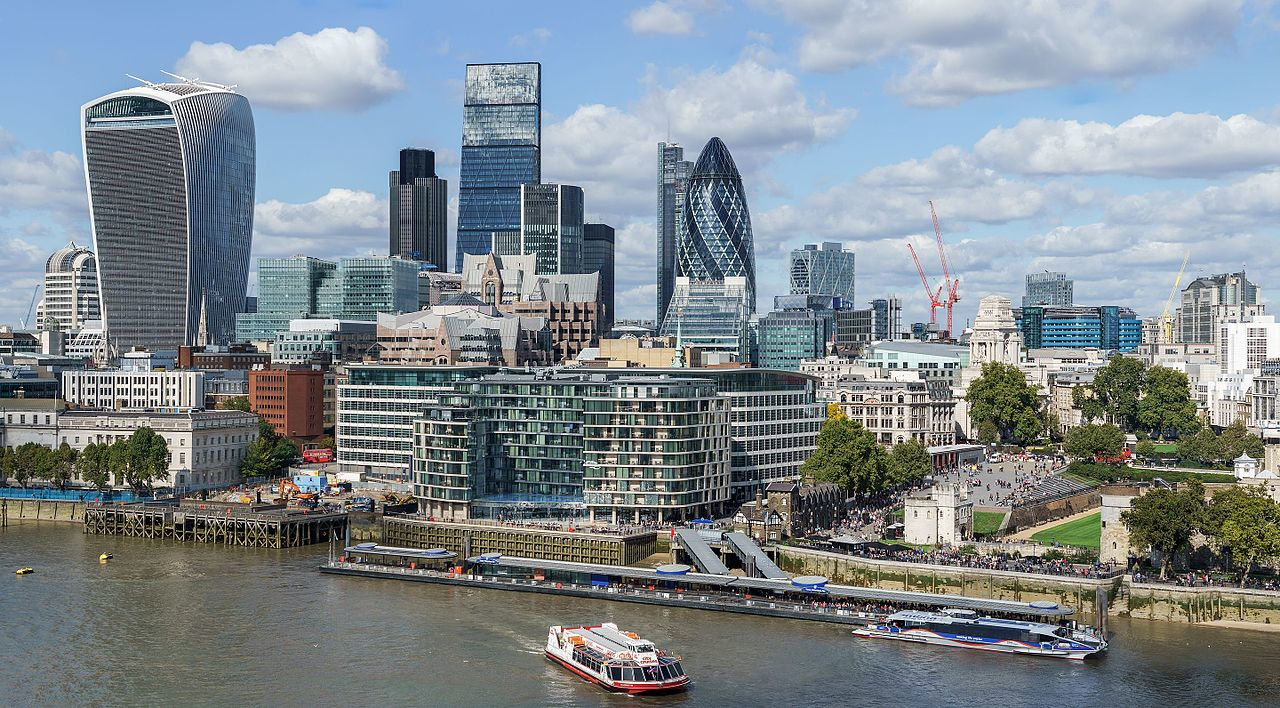
\includegraphics[height=\textheight]{images/city-of-london}
\end{center}
\hltfootnote
}


\frame{
\begin{center}
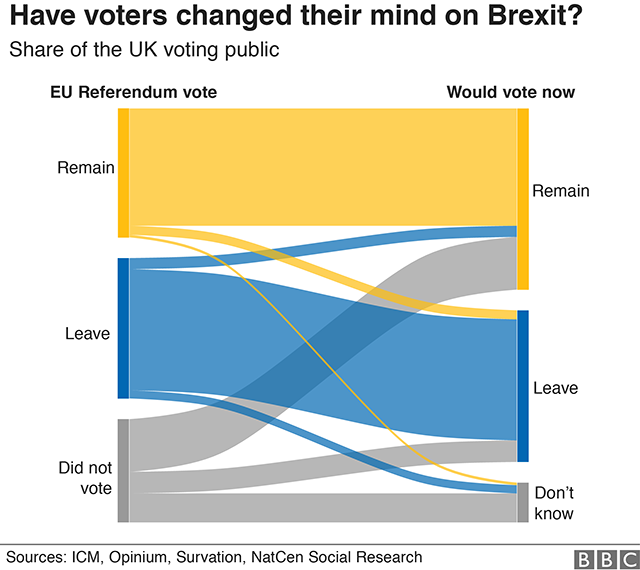
\includegraphics[height=.9\textheight]{images/brexit-change-of-mind.png}
\end{center}
\vspace{1em}
\footnotesize{Source: BBC}
}

\frame{}

\section*{Conclusions}

\frame{

\frametitle{Conclusions}

\begin{itemize}\itemsep1em
\item<2-> Leave voters were older, more rural, less education, and opposed to rising immigration

\item<3-> Remain voters were younger, more urban, more likely to have attended university

\item<4-> Voters divided on what they want from Britain and views of what impact it will have

\item<5-> Britain is leaving the EU, but the type of Brexit remains unknown
\end{itemize}

}


\frame{
\begin{center}
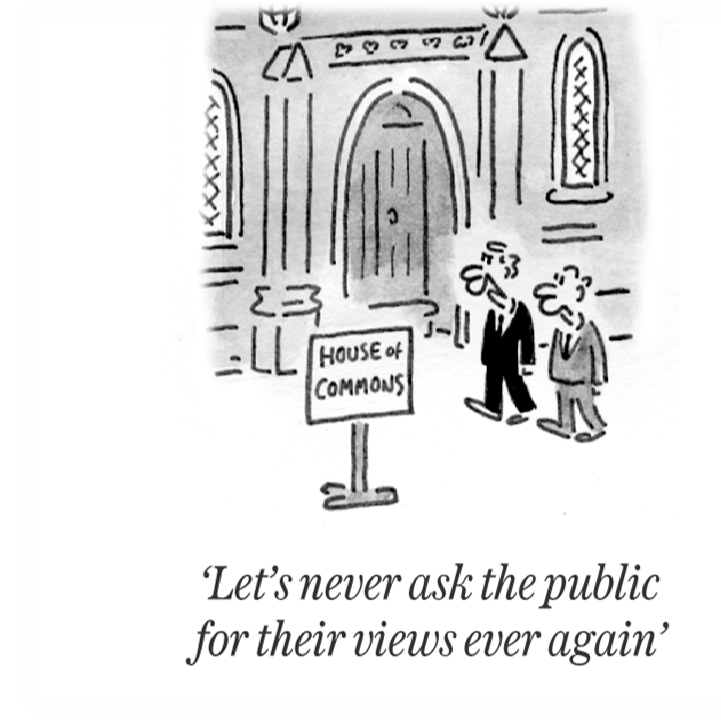
\includegraphics[height=.9\textheight]{images/cartoon}
\end{center}
}


\bgroup
\setbeamercolor{background canvas}{bg=white}
\begin{frame}[plain]
\begin{center}

\includegraphics[height=.9\textheight]{images/lse-beaver}
\end{center}
\end{frame}
\egroup


\bgroup
\setbeamercolor{background canvas}{bg=black}
\setbeamertemplate{background}
{
\includegraphics[height=\paperheight,width=\paperwidth]{images/black.png}}
\begin{frame}[plain]{}
\end{frame}
\egroup

\appendix

\end{document}
